\documentclass[journal,12pt,twocolumn]{IEEEtran}
%
\usepackage{setspace}
\usepackage{gensymb}
%\doublespacing
\singlespacing

%\usepackage{graphicx}
%\usepackage{amssymb}
%\usepackage{relsize}
\usepackage[cmex10]{amsmath}
\usepackage{siunitx}
%\usepackage{amsthm}
%\interdisplaylinepenalty=2500
%\savesymbol{iint}
%\usepackage{txfonts}
%\restoresymbol{TXF}{iint}
%\usepackage{wasysym}
\usepackage{amsthm}
\usepackage{iithtlc}
\usepackage{mathrsfs}
\usepackage{txfonts}
\usepackage{stfloats}
\usepackage{steinmetz}
%\usepackage{bm}
\usepackage{cite}
\usepackage{cases}
\usepackage{subfig}
%\usepackage{xtab}
\usepackage{longtable}
\usepackage{multirow}
%\usepackage{algorithm}
%\usepackage{algpseudocode}
\usepackage{enumitem}
\usepackage{mathtools}
\usepackage{tikz}
\usepackage{circuitikz}
\usepackage{pgfplots}
\usepackage{verbatim}
\usepackage{tfrupee}
\usepackage[breaklinks=true]{hyperref}
%\usepackage{stmaryrd}
\usepackage{tkz-euclide} % loads  TikZ and tkz-base
%\usetkzobj{all}
\usetikzlibrary{calc,math}
\usetikzlibrary{fadings}
\usepackage{listings}
    \usepackage{color}                                            %%
    \usepackage{array}                                            %%
    \usepackage{longtable}                                        %%
    \usepackage{calc}                                             %%
    \usepackage{multirow}                                         %%
    \usepackage{hhline}                                           %%
    \usepackage{ifthen}                                           %%
  %optionally (for landscape tables embedded in another document): %%
    \usepackage{lscape}     
\usepackage{multicol}
\usepackage{chngcntr}
%\usepackage{enumerate}

%\usepackage{wasysym}
%\newcounter{MYtempeqncnt}
\DeclareMathOperator*{\Res}{Res}
%\renewcommand{\baselinestretch}{2}
\renewcommand\thesection{\arabic{section}}
\renewcommand\thesubsection{\thesection.\arabic{subsection}}
\renewcommand\thesubsubsection{\thesubsection.\arabic{subsubsection}}

\renewcommand\thesectiondis{\arabic{section}}
\renewcommand\thesubsectiondis{\thesectiondis.\arabic{subsection}}
\renewcommand\thesubsubsectiondis{\thesubsectiondis.\arabic{subsubsection}}

% correct bad hyphenation here
\hyphenation{op-tical net-works semi-conduc-tor}
\def\inputGnumericTable{}                                 %%

\lstset{
%language=C,
frame=single, 
breaklines=true,
columns=fullflexible
}
%\lstset{
%language=tex,
%frame=single, 
%breaklines=true
%}

\begin{document}
%


\newtheorem{theorem}{Theorem}[section]
\newtheorem{problem}{Problem}
\newtheorem{proposition}{Proposition}[section]
\newtheorem{lemma}{Lemma}[section]
\newtheorem{corollary}[theorem]{Corollary}
\newtheorem{example}{Example}[section]
\newtheorem{definition}[problem]{Definition}
%\newtheorem{thm}{Theorem}[section] 
%\newtheorem{defn}[thm]{Definition}
%\newtheorem{algorithm}{Algorithm}[section]
%\newtheorem{cor}{Corollary}
\newcommand{\BEQA}{\begin{eqnarray}}
\newcommand{\EEQA}{\end{eqnarray}}
\newcommand{\define}{\stackrel{\triangle}{=}}

\bibliographystyle{IEEEtran}
%\bibliographystyle{ieeetr}


\providecommand{\mbf}{\mathbf}
\providecommand{\pr}[1]{\ensuremath{\Pr\left(#1\right)}}
\providecommand{\qfunc}[1]{\ensuremath{Q\left(#1\right)}}
\providecommand{\sbrak}[1]{\ensuremath{{}\left[#1\right]}}
\providecommand{\lsbrak}[1]{\ensuremath{{}\left[#1\right.}}
\providecommand{\rsbrak}[1]{\ensuremath{{}\left.#1\right]}}
\providecommand{\brak}[1]{\ensuremath{\left(#1\right)}}
\providecommand{\lbrak}[1]{\ensuremath{\left(#1\right.}}
\providecommand{\rbrak}[1]{\ensuremath{\left.#1\right)}}
\providecommand{\cbrak}[1]{\ensuremath{\left\{#1\right\}}}
\providecommand{\lcbrak}[1]{\ensuremath{\left\{#1\right.}}
\providecommand{\rcbrak}[1]{\ensuremath{\left.#1\right\}}}
\theoremstyle{remark}
\newtheorem{rem}{Remark}
\newcommand{\sgn}{\mathop{\mathrm{sgn}}}
\providecommand{\abs}[1]{\left\vert#1\right\vert}
\providecommand{\res}[1]{\Res\displaylimits_{#1}} 
\providecommand{\norm}[1]{\left\lVert#1\right\rVert}
%\providecommand{\norm}[1]{\lVert#1\rVert}
\providecommand{\mtx}[1]{\mathbf{#1}}
\providecommand{\mean}[1]{E\left[ #1 \right]}
\providecommand{\fourier}{\overset{\mathcal{F}}{ \rightleftharpoons}}
%\providecommand{\hilbert}{\overset{\mathcal{H}}{ \rightleftharpoons}}
\providecommand{\ztrans}{\overset{\mathcal{Z}}{ \rightleftharpoons}}
\providecommand{\system}{\overset{\mathcal{H}}{ \longleftrightarrow}}
	%\newcommand{\solution}[2]{\textbf{Solution:}{#1}}
\newcommand{\solution}{\noindent \textbf{Solution: }}
\newcommand{\cosec}{\,\text{cosec}\,}
\providecommand{\dec}[2]{\ensuremath{\overset{#1}{\underset{#2}{\gtrless}}}}
\newcommand{\myvec}[1]{\ensuremath{\begin{pmatrix}#1\end{pmatrix}}}
\newcommand{\mydet}[1]{\ensuremath{\begin{vmatrix}#1\end{vmatrix}}}
\providecommand{\gauss}[2]{\mathcal{N}\ensuremath{\left(#1,#2\right)}}
%\providecommand{\system}[1]{\overset{\mathcal{#1}}{ \longleftrightarrow}}
\newcommand*{\permcomb}[4][0mu]{{{}^{#3}\mkern#1#2_{#4}}}
\newcommand*{\perm}[1][-3mu]{\permcomb[#1]{P}}
\newcommand*{\comb}[1][-1mu]{\permcomb[#1]{C}}
%\numberwithin{equation}{section}
\numberwithin{equation}{subsection}
%\numberwithin{problem}{section}
%\numberwithin{definition}{section}
\makeatletter
\@addtoreset{figure}{problem}
\makeatother

\let\StandardTheFigure\thefigure
\let\vec\mathbf
%\renewcommand{\thefigure}{\theproblem.\arabic{figure}}
\renewcommand{\thefigure}{\theproblem}
%\setlist[enumerate,1]{before=\renewcommand\theequation{\theenumi.\arabic{equation}}
%\counterwithin{equation}{enumi}


%\renewcommand{\theequation}{\arabic{subsection}.\arabic{equation}}

\def\putbox#1#2#3{\makebox[0in][l]{\makebox[#1][l]{}\raisebox{\baselineskip}[0in][0in]{\raisebox{#2}[0in][0in]{#3}}}}
     \def\rightbox#1{\makebox[0in][r]{#1}}
     \def\centbox#1{\makebox[0in]{#1}}
     \def\topbox#1{\raisebox{-\baselineskip}[0in][0in]{#1}}
     \def\midbox#1{\raisebox{-0.5\baselineskip}[0in][0in]{#1}}

\vspace{3cm}

\title{
%	\logo{
Probability and Random Variables
%	}
}
\author{ G V V Sharma$^{*}$% <-this % stops a space
	\thanks{*The author is with the Department
		of Electrical Engineering, Indian Institute of Technology, Hyderabad
		502285 India e-mail:  gadepall@iith.ac.in. All content in this manual is released under GNU GPL.  Free and open source.}
	
}	
%\title{
%	\logo{Matrix Analysis through Octave}{\begin{center}\includegraphics[scale=.24]{tlc}\end{center}}{}{HAMDSP}
%}


% paper title
% can use linebreaks \\ within to get better formatting as desired
%\title{Matrix Analysis through Octave}
%
%
% author names and IEEE memberships
% note positions of commas and nonbreaking spaces ( ~ ) LaTeX will not break
% a structure at a ~ so this keeps an author's name from being broken across
% two lines.
% use \thanks{} to gain access to the first footnote area
% a separate \thanks must be used for each paragraph as LaTeX2e's \thanks
% was not built to handle multiple paragraphs
%

%\author{<-this % stops a space
%\thanks{}}
%}
% note the % following the last \IEEEmembership and also \thanks - 
% these prevent an unwanted space from occurring between the last author name
% and the end of the author line. i.e., if you had this:
% 
% \author{....lastname \thanks{...} \thanks{...} }
%                     ^------------^------------^----Do not want these spaces!
%
% a space would be appended to the last name and could cause every name on that
% line to be shifted left slightly. This is one of those "LaTeX things". For
% instance, "\textbf{A} \textbf{B}" will typeset as "A B" not "AB". To get
% "AB" then you have to do: "\textbf{A}\textbf{B}"
% \thanks is no different in this regard, so shield the last } of each \thanks
% that ends a line with a % and do not let a space in before the next \thanks.
% Spaces after \IEEEmembership other than the last one are OK (and needed) as
% you are supposed to have spaces between the names. For what it is worth,
% this is a minor point as most people would not even notice if the said evil
% space somehow managed to creep in.



% The paper headers
%\markboth{Journal of \LaTeX\ Class Files,~Vol.~6, No.~1, January~2007}%
%{Shell \MakeLowercase{\textit{et al.}}: Bare Demo of IEEEtran.cls for Journals}
% The only time the second header will appear is for the odd numbered pages
% after the title page when using the twoside option.
% 
% *** Note that you probably will NOT want to include the author's ***
% *** name in the headers of peer review papers.                   ***
% You can use \ifCLASSOPTIONpeerreview for conditional compilation here if
% you desire.




% If you want to put a publisher's ID mark on the page you can do it like
% this:
%\IEEEpubid{0000--0000/00\$00.00~\copyright~2007 IEEE}
% Remember, if you use this you must call \IEEEpubidadjcol in the second
% column for its text to clear the IEEEpubid mark.



% make the title area
\maketitle

\newpage

\tableofcontents

\bigskip

\renewcommand{\thefigure}{\theenumi}
\renewcommand{\thetable}{\theenumi}
%\renewcommand{\theequation}{\theenumi}

%\begin{abstract}
%%\boldmath
%In this letter, an algorithm for evaluating the exact analytical bit error rate  (BER)  for the piecewise linear (PL) combiner for  multiple relays is presented. Previous results were available only for upto three relays. The algorithm is unique in the sense that  the actual mathematical expressions, that are prohibitively large, need not be explicitly obtained. The diversity gain due to multiple relays is shown through plots of the analytical BER, well supported by simulations. 
%
%\end{abstract}
% IEEEtran.cls defaults to using nonbold math in the Abstract.
% This preserves the distinction between vectors and scalars. However,
% if the journal you are submitting to favors bold math in the abstract,
% then you can use LaTeX's standard command \boldmath at the very start
% of the abstract to achieve this. Many IEEE journals frown on math
% in the abstract anyway.

% Note that keywords are not normally used for peerreview papers.
%\begin{IEEEkeywords}
%Cooperative diversity, decode and forward, piecewise linear
%\end{IEEEkeywords}



% For peer review papers, you can put extra information on the cover
% page as needed:
% \ifCLASSOPTIONpeerreview
% \begin{center} \bfseries EDICS Category: 3-BBND \end{center}
% \fi
%
% For peerreview papers, this IEEEtran command inserts a page break and
% creates the second title. It will be ignored for other modes.
%\IEEEpeerreviewmaketitle

\begin{abstract}
This book provides a simple introduction to probability and random variables.   The contents are largely based on  NCERT textbooks from Class 9-12.
\end{abstract}


\section{Axioms of Probability}
\subsection{Boolean Logic}
If A and B are two events such that $\pr{A} = \frac{1}{4}, \pr{B} = \frac{1}{2}$ and $\pr{A B} = \frac{1}{8}$. find $\pr{\text{not A and not B}}$.
\renewcommand{\theequation}{\theenumi}
\begin{enumerate}[label=\thesubsection.\arabic*.,ref=\thesubsection.\theenumi]
\numberwithin{equation}{enumi}

\item 
\begin{align}
A^{\prime}B^{\prime} &=  \brak{A+B}^{\prime}
\\
\implies \pr{A^{\prime}B^{\prime}} &=  \pr{\brak{A+B}^{\prime}} 
\\
&= 1 - \pr{A+B} 
\label{eq:axiom_sum_one}
\end{align}
\item 
\begin{align}
\because A+B &= A\brak{B+B^{\prime}} + B
\\
&= B \brak{A +1} + A B^{\prime}
\\
&=B + A B^{\prime}
\\
\implies \pr{A+B} &= \pr{B + A B^{\prime} }
\\
&=\pr{B}+\pr{ A B^{\prime} } 
\\
&\because B \brak{ A B^{\prime} } = 0
\label{eq:axiom_sum_two}
\end{align}
\item 
\begin{align}
A = A \brak{B+B^{\prime}} =  AB + AB^{\prime}
\label{eq:axiom_sum_A}
\end{align}
and 
\begin{align}
\brak{ AB}\brak{  AB^{\prime}} = 0, \because BB^{\prime} = 0
\label{eq:axiom_sum_AB0}
\end{align}
Hence, $AB$ and $AB^{\prime}$ are mutually exclusive and 
%
\begin{align}
\pr{A} = \pr{AB} + \pr{AB^{\prime}}
\\
\implies 
\pr{AB^{\prime}} =  \pr{A} - \pr{AB}
\label{eq:axiom_sum_ABp}
\end{align}
\item Substituting \eqref{eq:axiom_sum_ABp} in \eqref{eq:axiom_sum_two}, 
\begin{align}
\pr{A+B} &= \pr{A} + \pr{B} - \pr{AB} 
\label{eq:axiom_sum_AB}
\end{align}
\item Substituting \eqref{eq:axiom_sum_AB} in \eqref{eq:axiom_sum_one}
\begin{align}
\pr{A^{\prime}B^{\prime}} &=  1 - \cbrak{\pr{A} + \pr{B} - \pr{AB} }
\\
&= 1 - \brak{\frac{1}{4} + \frac{1}{2} - \frac{1}{8}}
\\
&= \frac{3}{8}
\label{eq:axiom_sum_final}
\end{align}
\end{enumerate}
\subsection{Independent Events}
\renewcommand{\theequation}{\theenumi}
\begin{enumerate}[label=\thesubsection.\arabic*.,ref=\thesubsection.\theenumi]
\numberwithin{equation}{enumi}



\item Prove that if $E$ and $F$ are independent events, then so are the events $E$ and $F^{\prime}$.\\
\solution  If $E$ and $F$ are independent,
\begin{align}
\pr{EF} = \pr{E}\pr{F}
\label{eq:axiom_indep}
\end{align}
From 
\eqref{eq:axiom_sum_AB0}
%
\begin{align}
\pr{EF^{\prime}} =  \pr{E} - \pr{EF}
\label{eq:axiom_indep_EFp}
\end{align}
Substituting from \eqref{eq:axiom_indep} in \eqref{eq:axiom_indep_EFp},
%
\begin{align}
\pr{EF^{\prime}} &=  \pr{E} \brak{1- \pr{F}}
&= \pr{E} \pr{F^{\prime}}
\label{eq:axiom_indep_EFp_ind}
\end{align}
%
\begin{align}
\because FF^{\prime} = 0, F + F^{\prime} = 1
\\
\implies \pr{F}+\pr{F^{\prime}} = 1
\label{eq:axiom_FFp}
\end{align}
By definition, from \eqref{eq:axiom_indep_EFp_ind}, we conclude that $E$ and $F^{\prime}$ are independent.
\item If A and B are two independent events, then the probability of occurrence of at least one of A and B is given by 1- $P(A^{\prime}) P(B^{\prime})$\\
\solution 
\begin{align}
\because (A+B)(A+B)^{\prime} = 0
\\
\implies 1 = \pr{A+B} + \pr{\brak{A+B}^{\prime}}
\\
\implies \pr{A+B} = 1 - \pr{A^{\prime}B^{\prime}} 
\\
= 1 - \pr{A^{\prime}}\pr{B^{\prime}} 
\end{align}
using the definition of independence.
\end{enumerate}
\subsection{Conditional Probability}
\renewcommand{\theequation}{\theenumi}
\begin{enumerate}[label=\thesubsection.\arabic*.,ref=\thesubsection.\theenumi]
\numberwithin{equation}{enumi}

\item Given that E and F are events such that P(E) = 0.6, P(F) = 0.3 and P(E  F) = 0.2, find $\pr{E|F}$ and $\pr{F|E}$\\
\solution By definition,
\begin{align}
\pr{E|F} = \frac{\pr{EF}}{\pr{F}} = \frac{0.2}{0.3} = \frac{2}{3}
\end{align}
%
Similarly,
\begin{align}
\pr{F|E} = \frac{\pr{EF}}{\pr{E}} = \frac{1}{3}
\end{align}


\item A fair die is rolled. Consider the events E =  (1, 3, 5), F = (2, 3) and G = (2, 3, 4, 5) Find\\
\begin{enumerate}
\item  $\pr{E|F}$ and $\pr{F|E}$
\item  $\pr{E|G}$ and  $\pr{F|E}$
\item   $\pr{\brak{E+F}|G}$ and  $\pr{EF|G}$ 
\end{enumerate}
\solution
%\input{./solutions/docq22.tex}

From the given information,
	\begin{align}
	\pr{E} &= \frac{3}{6} = \frac{1}{2} \\
	\pr{F} &= \frac{2}{6} = \frac{1}{3} \\	
	\pr{G} &= \frac{4}{6} = \frac{2}{3} \\	
	\pr{E F} &= \frac{1}{6}\\
	\pr{E G} &= \frac{2}{6}= \frac{1}{3}\\
	\pr{F G} &= \frac{2}{6}= \frac{1}{3}\\
	\pr{E F G} &= \frac{1}{6}
\end{align}
\begin{enumerate}
\item	
\begin{align}
	\pr{E|F} &= \frac{\pr{E F}}{\pr{F}}\\
	\pr{E|F} &= \frac{\frac{1}{6}}{\frac{1}{3}} = \frac{1}{2}\\
	\pr{F|E} &= \frac{\pr{F E}}{\pr{E}}\\
	\pr{F|E} &= \frac{\frac{1}{6}}{\frac{1}{2}} = \frac{1}{3}
	\end{align}

\item 	\begin{align}
	\pr{E|G} &= \frac{\pr{E G}}{\pr{G}}\\
	\pr{E|G} &= \frac{\frac{1}{3}}{\frac{2}{3}} = \frac{1}{2}\\
	\pr{G|E} &= \frac{\pr{G E}}{\pr{G}}\\
	\pr{G|E} &= \frac{\frac{1}{3}}{\frac{1}{2}} = \frac{2}{3}\\
	\end{align}
	
\item	%$\pr{\frac{E\cup F}{G}}$
\begin{multline}
\pr{E+F|G} = \frac{\pr{\cbrak{E+F}G}}{\pr{G}}
\\
 = \frac{\pr{EG + FG}}{\pr{G}}
\\
=\frac{\pr{EG} +\pr{ FG}- \pr{EFG}}{\pr{G}}
\\
 = \frac{3}{4}
\end{multline}
and 
\begin{align}
\pr{EF|G} = 
\frac{ \pr{EFG}}{\pr{G}}
 = \frac{1}{4}
\end{align}

\end{enumerate}


\end{enumerate}



\section{Sum of Independent Random Variables}
\subsection{The Uniform Distribution}
\input{./chapters/sum.tex}
\section{Cumulative Distribution Function}
\subsection{The Bernoulli Distribution}
\renewcommand{\theequation}{\theenumi}
\begin{enumerate}[label=\thesection.\arabic*.,ref=\thesection.\theenumi]
\numberwithin{equation}{enumi}


\item A jar contains 24 marbles, some are green and others are blue. If a marble is drawn at random from the jar, the probability that it is green is $\frac{2}{3}$. Find the number of blue balls in the jar.
\\
\solution
 Let the random variable $X = \{ 0,1 \}$ denote the outcome of the given experiment.
\\$X = 1$ if the marble picked turns out $Green$.
\\$X = 0$ if the marble picked turns out $Blue$.
\\It is given that,
\begin{align}
P(X = 1) &= \frac{2}{3}\\
\implies P(X = 0) &= 1 - P(X = 1)\\
\implies P(X = 0) &= 1 - \frac{2}{3}\\
\implies P(X = 0) &= \frac{1}{3}
\end{align}
Now
\begin{align}
n(X = 0) + n(X = 1) &= 24\\
\because P(X = 0) &= \frac{n(X = 0)}{n(X = 0) + n(X = 1)},\\
 n(X = 0) &= P(X = 0)\left(n(X = 0) + n(X = 1)\right)\\
\implies n(X = 0) &= \frac{(1)\times (24)}{3}\\
\implies n(X = 0) &= 8
\end{align}
$\therefore{}$ the  number of blue balls is 8.

\item A bag contains lemon flavoured candies only. Malini takes out one candy without
looking into the bag. What is the probability that she takes out\\
(i) an orange flavoured candy?\\
(ii) a lemon flavoured candy?
\solution  Let the random variable $X=\{0,1\}$ represent the outcome of the flavour of the candy Malini picks. $X=0$ denotes an orange flavoured candy, while $X=1$ denotes a lemon flavoured candy.  Then 
\begin{align}
\pr{X=0} = 1,
\\
\pr{X=1} = 0
\end{align}
\item 
\item 
\item 
\item 
\item 
\item A person buys a lottery ticket in 50 lotteries, in each of which his chance of
winning a prize is $\frac{1}{100}$.What is the probability that he will win a prize\\
(a) at least once \\
(b) exactly once \\
(c) at least twice?\\
From the given information, the random variable representing the trials is
\begin{align}
X \sim B\brak{50,\frac{1}{100}}
\end{align}
%
Hence the desired probabilites are
\begin{enumerate}
\item 
\begin{align}
\pr{X \ge 1} = 1 - \pr{X =0} = 1-\brak{\frac{99}{100}}^{50} 
\end{align}
%
\item 
\begin{align}
\pr{X = 1} = {50}\brak{\frac{99}{100}}^{49} \brak{\frac{1}{100}}
\end{align}
%
\item 
\begin{align}
\pr{X \ge 2} &= 1 - \pr{X \le 1} 
\\
&= 1 - \pr{X =0} - \pr{X = 1} \\
&= 1 -\brak{\frac{149}{100}}\brak{\frac{99}{100}}^{49}\\
&= 0.0894
\end{align}

\end{enumerate}


\item In an examination, 20 questions of true-false type are asked. Suppose a student tosses a fair coin to determine his answer to each question. If the coin falls heads, he answers 'true'; if it falls tails, he answers 'false'. Find the probability that he answers at least 12 questions correctly.\\
\solution
Let X be the number of correct answers\\
n be the number of questions $(n=20)$\\
p is the probability of correct answer $(p=0.5)$\\
q is the probability of wrong answer $(q=1-p)$
From Bernoulli's distribution,
\begin{align}
    \pr{X=r}&=\comb{n}{r}p^rq^{n-r}
\end{align}
$\therefore$ required probability is
\begin{align}
    \pr{X\geq12}&=\sum_{r=12}^{n}\comb{n}{r} p^r q^{n-r}\\
    &=\sum_{r=12}^{20}\comb{20}{r} p^r (1-p)^{20-r}\\
    &=0.25172233581
\end{align}

\item There are 5$\%$ defective items in a large bulk of items. What is the probability
that a sample of 10 items will include not more than one defective item?\\
\solution
Let X be the random variable representing all the items.  Then,
\begin{align}
X = \sum_{i=1}^{10}X_i
\end{align}
%
has a Binomial distribution with
$X_i \in \cbrak{0,1}$ being a Bernoulli r.v. representing the item condition.  From the given information, the probability of an item being
defective is given by
\begin{align}
\pr{X_i = 0} &= \frac{1}{20} = p
\\
\implies \pr{X_i = 1} &= q = 1-p =  1-\frac{1}{20} = \frac{19}{20}
\end{align}
%
$\because$
 \begin{align}
    X &\sim B(n=10,p=0.5),
    \\
   \pr{X=r}&=    \comb{n}{r} p^r q^{n-r}
   \end{align}
\begin{multline}
\implies Pr(X \le 1)=Pr(X=0)+Pr(X=1) \\
              =\comb{10}{0}\left(\frac{1}{20}\right)^0 \left(\frac{19}{20}\right)^{10}+\comb{10}{1} \left(\frac{1}{20}\right)^1 \left(\frac{19}{20}\right)^{9}\\
              =\left(\frac{29}{20}\right) \times\left (\frac{19}{20}\right) ^{9}
              =0.9138
\end{multline} 



\item In a meeting, 70$\%$ of the members favour and 30$\%$ oppose a certain proposal.
A member is selected at random and we take X = 0 if he opposed, and X = 1 if he is in favour. Find E(X) and Var (X).\\
\solution
From the given information,
\begin{align}
\pr{X=0} = 70 {\%} = 0.7\\
\pr{X=1} = 30 {\%} =0.3
\end{align}
Hence,
\begin{align}
    E(X) &= 1\times0.7 + 0\times0.3 =0.7
    \\
    E(X^2) &= 1^2\times0.7 + 0^2\times0.3 =0.7
    \\
    \implies Var(X) &= E(X^2) -[E(X)]^2
    \\&= 0.7- 0.7^2 = 0.21
\end{align}

\item A coin is biased so that the head is 3 times as likely to occur as tail. If the coin is tossed twice, find the probability distribution of number of tails.\\
\item From a lot of 30 bulbs which include 6 defectives, a sample of 4 bulbs is drawn at random with replacement. Find the probability distribution of the number of defective bulbs.\\
\item Probability that A speaks truth is $\frac{4}{5}$. A coin is tossed. A reports that a head appears. The probability that actually there was head is\\
\begin{enumerate}
\item $\frac{4}{5}$
\item $\frac{1}{2}$
\item $\frac{1}{5}$
\item $\frac{2}{5}$
\end{enumerate}
\solution
Let X $\in\{0,1\}$ be the random variable denoting that A tells truth when X=1

\begin{align*}
\tag{1.14.1}
     \Pr(X=1)=\frac{4}{5}\\
      \Pr(X=0)=1-\Pr(X=1)
\end{align*}
\begin{align}
\tag{1.14.2}
    \Pr(X=0) =\frac{1}{5}
\end{align}
Let Y $\in\{0,1\}$ be the random variable denoting that Head appears on the coin when Y=1 \\
As the coin is unbiased,\\
\begin{align}
\tag{1.14.3}
    \Pr(Y=1|X=1)=\frac{1}{2}
\end{align}
\begin{align}
\tag{1.14.4}
    \Pr(Y=1|X=0)=\frac{1}{2}
\end{align}
Probability that actually there was a head given that A reports a Head\\
=$\Pr(X=1|Y=1)$

From Bayes Theorm,

\begin{align*}
    &\Pr(X=1|Y=1)=\frac{\Pr(X=1)\times\Pr(Y=1|X=1)}{\sum_{i=0}^{1}\Pr(X=i)\times\Pr(Y=1|X=i)}\\
   &=\frac{\frac{4}{5}\times\frac{1}{2}}{\frac{4}{5}\times\frac{1}{2}+\frac{1}{5}\times\frac{1}{2}}\\
    &=\frac{4}{5}
\end{align*}
Probability that  actually there was a head given that A reports a Head=$\frac{4}{5}$\\
So, option a) is correct.

\item A box of oranges is inspected by examining three randomly selected oranges drawn without replacement. If all the three oranges are good, the box is approved for sale, otherwise, it is rejected. Find the probability that a box containing 15 oranges out of which 12 are good and 3 are bad ones will be approved for sale.\\
\solution
%
Let the $i$th inspection be $X_i \in \cbrak{0,1}$, where  1 represents a good orange.  From the given information,
\begin{align}
\pr{X_1=1}&=\brak{\frac{12}{15}}\\ 
\pr{X_2=1|X_1=1}&=\brak{\frac{11}{14}} \\ 
\pr{X_3=1|X_1=1,X_2=1} &= \brak{\frac{10}{13}}
\end{align}
%
The probability that the box will be approved for sale is
\begin{multline}
\pr{X_1=1,X_2=1,X_3=1} 
\\
= \pr{X_1=1} \times \pr{X_2=1|X_1=1} 
\\
\times \pr{X_3=1|X_1=1,X_2=1} \\ 
=\frac{12}{15}\times \frac{11}{14} \times \frac{10}{13}\\ 
=\frac{1320}{2730} =0.483 
\end{multline}
%
\item Determine P(E/F), if a coin is tossed three times\\
(i) E : head on third toss , F : heads on first two tosses\\
(ii) E : at least two heads , F : at most two heads\\
(iii) E : at most two tails , F : at least one tail\\
%
\solution
In an experiment of tossing a coin $n$( = 3) times, random variable  $X \in \lbrace 0,1,2,3 \rbrace$ follows binomial distribution.\\
The binomial distribution formula is:
\begin{align*}
 \Pr( X=k ) &= \comb{n}{k} \times p^k \times (1- p)^{n - k}
\end{align*}

Where:


\begin{table}[h]

    \centering
    \resizebox{\columnwidth}{!}{%
    \begin{tabular}{|r|c|}\hline
    $k$ &  total number of “successes” \\ \hline
    $p$ & probability of a success on an individual trial\\ \hline
    $n$ & number of trials = 3 \\ \hline
\end{tabular}}
\caption{The binomial distribution formula}
    \label{1.16:table:0}
\end{table}


\begin{enumerate}[label=(\roman*)]
    \item From table \ref{1.16:table:1}, $\Pr(E|F)$ = 0.5
    \item $X$ denotes number of heads. From table \ref{1.16:table:2}, $\Pr(E|F)$ = 0.428
    \item $X$ denotes number of tails. From table \ref{1.16:table:3}, $\Pr(E|F)$ = 0.857
\end{enumerate}


\begin{table}[ht]

    \centering
     \resizebox{\columnwidth}{!}{%
    \begin{tabular}{|r|l|} \hline
    $\Pr$(Event)  & Calculation   \\ \hline
    $\Pr( F)$    & From product rule , \\ 
    &= $\frac{1}{2}\times\frac{1}{2}$ \\ 
    &=  0.25 \\ \hline 
    $\Pr( EF)$   &  From product rule, \\   
    &= $\frac{1}{2}\times\frac{1}{2}\times\frac{1}{2}$ \\ 
    & = 0.125\\ \hline 
    $\Pr(E|F )$  &= $\frac{\Pr(EF)}{\Pr(F)} $ \\ 
    &  = 0.5 \\ \hline 
    \end{tabular} }
    \caption{Part(i)}
    \label{1.16:table:1}
\end{table}

\begin{table}[ht]

    \centering
    \resizebox{\columnwidth}{!}{%
     \begin{tabular}{|r|l|}\hline
      $\Pr$(Event)  & Calculation \\ \hline
      $\Pr( F)$ 
      &= $\Pr( X\leq2)$ \\ 
      &= $ \Pr( X=0) + \Pr( X=1) + \Pr( X=2 )$\\ 
      &= $\comb{3}{0} \left(\frac{1}{2}\right)^3  + \comb{3}{1} \left(\frac{1}{2}\right)^3 + \comb{3}{2} \left(\frac{1}{2}\right)^3$\\ 
      &= 0.875 \\ \hline
    $\Pr( EF)$  &= $\Pr( X=2) $ \\
    &= 0.375 \\ \hline
    $\Pr( E|F )$   &=$ \frac{\Pr(EF)}{\Pr(F)} $ \\ 
    &= 0.428 \\ \hline
    \end{tabular}}
    \caption{Part(ii)}
    \label{1.16:table:2}
\end{table}


\begin{table}[ht]

       \centering
       \resizebox{\columnwidth}{!}{%
       \begin{tabular}{|r|l|}\hline
      $\Pr$(Event)  & Calculation \\ \hline
       $\Pr( F)$ &= $\Pr( X\geq1)$\\
        &= $1-\Pr( 0)$ \\
        &= 0.875 \\ \hline
        $\Pr( EF)$ &= $\Pr(X= 1) + \Pr(X= 2 )$ \\
         &= 0.75 \\ \hline
         $\Pr( E|F)$ &= $\frac{\Pr(EF)}{\Pr(F)} $ \\
        &= 0.857 \\ \hline
      \end{tabular} }
       \caption{Part(iii)}
       \label{1.16:table:3}
   \end{table}
  


\item Determine P(E/F), if two coins are tossed once, where\\
(i) E : tail appears on one coin, F : one coin shows head\\
(ii) E : no tail appears, F : no head appears\\
%
\solution
Let X denote the number of heads shown on the coins, where n = 2 and p = 0.5, q = 1-p
\begin{align}
p(x) = \Pr(X=x) = \binom{n}{x}\times p^x\times q^{n-x}
\end{align}
\begin{table}[!ht]
\resizebox{\columnwidth}{!} {
\begin{tabular}{|c|c|c|c|}
\hline
     X&0&1&2  \\
     \hline
     P(X)&$\binom{2}{0}(0.5)^2=\dfrac{1}{4}$&$\binom{2}{1}(0.5)^2 = \dfrac{1}{2}$&$\binom{2}{2}(0.5)^2 = \dfrac{1}{4}$\\
     \hline
\end{tabular}
}
\caption{Probability of number of heads shown on the coins }
\label{1.17:table:1}
\end{table}
\begin{enumerate}
\item 
\begin{align}
&\Pr(F) = \Pr(X\geq 1)\\
&\Pr(F) = \Pr(X = 1) + \Pr(X = 2)\nonumber\\
       &= \frac{1}{2} + \frac{1}{4} = \frac{3}{4}\\
&\Pr(EF) = \Pr(X = 1) = \frac{1}{2}\\
&\Pr(E/F) =\frac{\Pr(EF)}{\Pr(F)} = \frac{2}{3}
\end{align}
\item
\begin{align}
&\Pr(F) = \Pr(X = 0) = \frac{1}{4}\\
&\Pr(EF) = 0\\
&\Pr(E/F) = \frac{\Pr(EF)}{\Pr(F)} = 0
\end{align} 
\end{enumerate}

\item Two players, Sangeeta and Reshma, play a tennis match. It is known
that the probability of Sangeeta winning the match is 0.62. What is the probability of
Reshma winning the match?
%
\\
\solution The desired probability is $1 - 0.62 = 0.38$.
\item Harpreet tosses two different coins simultaneously (say, one is of rupee 1
and other of rupee 2). What is the probability that she gets at least one head?

	\item In a cricket match, a batswoman hits a boundary 6 times out of 30 balls she plays. Find the probability that she did not hit a boundary.
\\
\solution
%
\begin{align}
    E(X) &= \frac{1}{\sqrt{2\pi}} \int_{-\infty}^{\infty} x e^{-\frac{x^2}{2}}dx\\
    &=0 \quad \brak{ \text{ odd function}}
\end{align}
\begin{align}
    E\brak{X^2}&= \frac{1}{\sqrt{2\pi}}\int_{-\infty}^{\infty} x^2
e^ {-\frac{x^2}{2}} dx \quad \brak{even function}\\
    &= \frac{2}{\sqrt{2\pi}} \int_{0}^{\infty} x^2 e^{-\frac{x^2}{2}} dx\\
    &= \frac{2}{\sqrt{2\pi}}\int_{0}^{\infty}\sqrt{2u}e^{-u} du \quad\brak{Let \frac{x^2}{2}= u}\\
    &= \frac{2}{\sqrt{\pi}} \int_{0}^{\infty} e^{-u} u^{\frac{3}{2}-1} du\\
    &= \frac{2}{\sqrt{\pi}} \Gamma\brak{{\frac{3}{2}}}\\
    &= \frac{1}{\sqrt{\pi}}\Gamma\brak{\frac{1}{2}} \\
    &= 1
\end{align}
where we have used the fact that
\begin{align}
\quad\because \Gamma(n)= (n-1)\Gamma(n-1); \Gamma\brak{\frac{1}{2}}=\sqrt{\pi}
\end{align}
%
Thus, the  variance is
\begin{align}
    \sigma^2 =  E\brak X^2 - E^2\brak X = 1
\end{align}

	\item A coin is tossed 1000 times with the following frequencies:\\
Head : 455, Tail : 545\\
Compute the probability for each event.\\
\solution
\input{./solutions/1-10/chapters/prob_exm/prob1/solution1.tex}
   \item Two coins are tossed simultaneously 500 times, and we get\\
       Two heads : 105 times\\
       One head : 275 times\\
       No head : 120 times\\
Find the probability of occurrence of each of these events.\\
\solution
\input{./solutions/1-10/chapters/prob_exm/prob2/solution2.tex}
   \item A die is thrown 1000 times with the frequencies for the outcomes 1, 2, 3, 4, 5 and 6 as given in the following Table \ref{table:prob_exam_3}.
Find the probability of getting each outcome.

\begin{table}[!ht]
\centering
\resizebox{\columnwidth}{!}{
\begin{tabular}{ |c|c|c|c|c|c|c| } 
 \hline
 \textbf{Outcome} &1 &2 &3 &4 &5 &6  \\ 
 \hline
 \textbf{Frequency} &179 &150 &157 &149 &175 &190 \\ 
 \hline
\end{tabular}
}
\caption{}
\label{table:prob_exam_3}
\end{table}
%\\
\solution
\input{./solutions/1-10/chapters/prob_exm/prob3/solution3.tex}

   \item The record of a weather station shows that out of the past 250 consecutive days, its weather forecasts were correct 175 times.\\
   (i) What is the probability that on a given day it was correct?\\
(ii) What is the probability that it was not correct on a given day?\\
\solution
\input{./solutions/1-10/chapters/prob_exm/prob5/solution5.tex}


\item {\em: Random Process}A and B throw a die alternatively till one of them gets a '6' and wins the game. Find their respective probabilities of winning, if A starts first.
\\
\solution
%
\begin{align}
    E(X) &= \frac{1}{\sqrt{2\pi}} \int_{-\infty}^{\infty} x e^{-\frac{x^2}{2}}dx\\
    &=0 \quad \brak{ \text{ odd function}}
\end{align}
\begin{align}
    E\brak{X^2}&= \frac{1}{\sqrt{2\pi}}\int_{-\infty}^{\infty} x^2
e^ {-\frac{x^2}{2}} dx \quad \brak{even function}\\
    &= \frac{2}{\sqrt{2\pi}} \int_{0}^{\infty} x^2 e^{-\frac{x^2}{2}} dx\\
    &= \frac{2}{\sqrt{2\pi}}\int_{0}^{\infty}\sqrt{2u}e^{-u} du \quad\brak{Let \frac{x^2}{2}= u}\\
    &= \frac{2}{\sqrt{\pi}} \int_{0}^{\infty} e^{-u} u^{\frac{3}{2}-1} du\\
    &= \frac{2}{\sqrt{\pi}} \Gamma\brak{{\frac{3}{2}}}\\
    &= \frac{1}{\sqrt{\pi}}\Gamma\brak{\frac{1}{2}} \\
    &= 1
\end{align}
where we have used the fact that
\begin{align}
\quad\because \Gamma(n)= (n-1)\Gamma(n-1); \Gamma\brak{\frac{1}{2}}=\sqrt{\pi}
\end{align}
%
Thus, the  variance is
\begin{align}
    \sigma^2 =  E\brak X^2 - E^2\brak X = 1
\end{align}

%
\item To know the opinion of the students about the subject statistics, a survey of 200 students was conducted. The data is recorded in Table \ref{table:1.2.6}
Find the probability that a student chosen at random
\begin{enumerate}
\item likes statistics,
\item  does not like it.
\end{enumerate}
\begin{table}[!ht]
\centering
\begin{tabular}{ |c|c| } 
 \hline
 \textbf{Opinion} &\textbf{Number of students}\\
 \hline
 like  &135\\ 
 \hline
 dislike  &65\\ 
 \hline
\end{tabular}
\caption{}
\label{table:1.2.6}
\end{table}
\solution
%
\begin{align}
    E(X) &= \frac{1}{\sqrt{2\pi}} \int_{-\infty}^{\infty} x e^{-\frac{x^2}{2}}dx\\
    &=0 \quad \brak{ \text{ odd function}}
\end{align}
\begin{align}
    E\brak{X^2}&= \frac{1}{\sqrt{2\pi}}\int_{-\infty}^{\infty} x^2
e^ {-\frac{x^2}{2}} dx \quad \brak{even function}\\
    &= \frac{2}{\sqrt{2\pi}} \int_{0}^{\infty} x^2 e^{-\frac{x^2}{2}} dx\\
    &= \frac{2}{\sqrt{2\pi}}\int_{0}^{\infty}\sqrt{2u}e^{-u} du \quad\brak{Let \frac{x^2}{2}= u}\\
    &= \frac{2}{\sqrt{\pi}} \int_{0}^{\infty} e^{-u} u^{\frac{3}{2}-1} du\\
    &= \frac{2}{\sqrt{\pi}} \Gamma\brak{{\frac{3}{2}}}\\
    &= \frac{1}{\sqrt{\pi}}\Gamma\brak{\frac{1}{2}} \\
    &= 1
\end{align}
where we have used the fact that
\begin{align}
\quad\because \Gamma(n)= (n-1)\Gamma(n-1); \Gamma\brak{\frac{1}{2}}=\sqrt{\pi}
\end{align}
%
Thus, the  variance is
\begin{align}
    \sigma^2 =  E\brak X^2 - E^2\brak X = 1
\end{align}

\item  Assume that each born child is equally likely to be a boy or a girl. If a family has two children, what is the conditional probability that both are girls given that\\
(i) the youngest is a girl,\\ 
(ii) at least one is a girl?\\
\solution
\input{./solutions/20-30/chapters/prob/exercises/docq23.tex}

\item  An instructor has a question bank consisting of 300 easy True / False questions,
200 difficult True / False questions, 500 easy multiple choice questions and 400 difficult multiple choice questions. If a question is selected at random from the question bank, what is the probability that it will be an easy question given that it is a multiple choice question?\\
\solution
\input{./solutions/20-30/chapters/prob/exercises/docq24.tex}
\item Two cards are drawn at random and without replacement from a pack of 52 playing cards. Find the probability that both the cards are black.\\
\solution
\input{./solutions/20-30/chapters/prob/exercises/docq30.tex}
\item Two balls are drawn at random with replacement from a box containing 10 black and 8 red balls. Find the probability that\\
(i) both balls are red.\\
(ii) first ball is black and second is red.\\
(iii) one of them is black and other is red.\\
\solution
%
\begin{align}
    E(X) &= \frac{1}{\sqrt{2\pi}} \int_{-\infty}^{\infty} x e^{-\frac{x^2}{2}}dx\\
    &=0 \quad \brak{ \text{ odd function}}
\end{align}
\begin{align}
    E\brak{X^2}&= \frac{1}{\sqrt{2\pi}}\int_{-\infty}^{\infty} x^2
e^ {-\frac{x^2}{2}} dx \quad \brak{even function}\\
    &= \frac{2}{\sqrt{2\pi}} \int_{0}^{\infty} x^2 e^{-\frac{x^2}{2}} dx\\
    &= \frac{2}{\sqrt{2\pi}}\int_{0}^{\infty}\sqrt{2u}e^{-u} du \quad\brak{Let \frac{x^2}{2}= u}\\
    &= \frac{2}{\sqrt{\pi}} \int_{0}^{\infty} e^{-u} u^{\frac{3}{2}-1} du\\
    &= \frac{2}{\sqrt{\pi}} \Gamma\brak{{\frac{3}{2}}}\\
    &= \frac{1}{\sqrt{\pi}}\Gamma\brak{\frac{1}{2}} \\
    &= 1
\end{align}
where we have used the fact that
\begin{align}
\quad\because \Gamma(n)= (n-1)\Gamma(n-1); \Gamma\brak{\frac{1}{2}}=\sqrt{\pi}
\end{align}
%
Thus, the  variance is
\begin{align}
    \sigma^2 =  E\brak X^2 - E^2\brak X = 1
\end{align}


\item Probability of solving specific problem independently by A and B are $\frac{1}{2}$
and $\frac{1}{3}$ respectively. If both try to solve the problem independently, find the probability that\\
(i) the problem is solved \\
(ii) exactly one of them solves the problem.\\
\solution
%
\begin{align}
    E(X) &= \frac{1}{\sqrt{2\pi}} \int_{-\infty}^{\infty} x e^{-\frac{x^2}{2}}dx\\
    &=0 \quad \brak{ \text{ odd function}}
\end{align}
\begin{align}
    E\brak{X^2}&= \frac{1}{\sqrt{2\pi}}\int_{-\infty}^{\infty} x^2
e^ {-\frac{x^2}{2}} dx \quad \brak{even function}\\
    &= \frac{2}{\sqrt{2\pi}} \int_{0}^{\infty} x^2 e^{-\frac{x^2}{2}} dx\\
    &= \frac{2}{\sqrt{2\pi}}\int_{0}^{\infty}\sqrt{2u}e^{-u} du \quad\brak{Let \frac{x^2}{2}= u}\\
    &= \frac{2}{\sqrt{\pi}} \int_{0}^{\infty} e^{-u} u^{\frac{3}{2}-1} du\\
    &= \frac{2}{\sqrt{\pi}} \Gamma\brak{{\frac{3}{2}}}\\
    &= \frac{1}{\sqrt{\pi}}\Gamma\brak{\frac{1}{2}} \\
    &= 1
\end{align}
where we have used the fact that
\begin{align}
\quad\because \Gamma(n)= (n-1)\Gamma(n-1); \Gamma\brak{\frac{1}{2}}=\sqrt{\pi}
\end{align}
%
Thus, the  variance is
\begin{align}
    \sigma^2 =  E\brak X^2 - E^2\brak X = 1
\end{align}

\item (i) A lot of 20 bulbs contain 4 defective ones. One bulb is drawn at random from the lot.
What is the probability that this bulb is defective?\\
(ii) Suppose the bulb drawn in (i) is not defective and is not replaced. Now one bulb
is drawn at random from the rest. What is the probability that this bulb is not
defective ?
\\
\solution
%
\begin{align}
    E(X) &= \frac{1}{\sqrt{2\pi}} \int_{-\infty}^{\infty} x e^{-\frac{x^2}{2}}dx\\
    &=0 \quad \brak{ \text{ odd function}}
\end{align}
\begin{align}
    E\brak{X^2}&= \frac{1}{\sqrt{2\pi}}\int_{-\infty}^{\infty} x^2
e^ {-\frac{x^2}{2}} dx \quad \brak{even function}\\
    &= \frac{2}{\sqrt{2\pi}} \int_{0}^{\infty} x^2 e^{-\frac{x^2}{2}} dx\\
    &= \frac{2}{\sqrt{2\pi}}\int_{0}^{\infty}\sqrt{2u}e^{-u} du \quad\brak{Let \frac{x^2}{2}= u}\\
    &= \frac{2}{\sqrt{\pi}} \int_{0}^{\infty} e^{-u} u^{\frac{3}{2}-1} du\\
    &= \frac{2}{\sqrt{\pi}} \Gamma\brak{{\frac{3}{2}}}\\
    &= \frac{1}{\sqrt{\pi}}\Gamma\brak{\frac{1}{2}} \\
    &= 1
\end{align}
where we have used the fact that
\begin{align}
\quad\because \Gamma(n)= (n-1)\Gamma(n-1); \Gamma\brak{\frac{1}{2}}=\sqrt{\pi}
\end{align}
%
Thus, the  variance is
\begin{align}
    \sigma^2 =  E\brak X^2 - E^2\brak X = 1
\end{align}

\item 12 defective pens are accidentally mixed with 132 good ones. It is not possible to just
look at a pen and tell whether or not it is defective. One pen is taken out at random from
this lot. Determine the probability that the pen taken out is a good one.
\\
\solution
%
\begin{align}
    E(X) &= \frac{1}{\sqrt{2\pi}} \int_{-\infty}^{\infty} x e^{-\frac{x^2}{2}}dx\\
    &=0 \quad \brak{ \text{ odd function}}
\end{align}
\begin{align}
    E\brak{X^2}&= \frac{1}{\sqrt{2\pi}}\int_{-\infty}^{\infty} x^2
e^ {-\frac{x^2}{2}} dx \quad \brak{even function}\\
    &= \frac{2}{\sqrt{2\pi}} \int_{0}^{\infty} x^2 e^{-\frac{x^2}{2}} dx\\
    &= \frac{2}{\sqrt{2\pi}}\int_{0}^{\infty}\sqrt{2u}e^{-u} du \quad\brak{Let \frac{x^2}{2}= u}\\
    &= \frac{2}{\sqrt{\pi}} \int_{0}^{\infty} e^{-u} u^{\frac{3}{2}-1} du\\
    &= \frac{2}{\sqrt{\pi}} \Gamma\brak{{\frac{3}{2}}}\\
    &= \frac{1}{\sqrt{\pi}}\Gamma\brak{\frac{1}{2}} \\
    &= 1
\end{align}
where we have used the fact that
\begin{align}
\quad\because \Gamma(n)= (n-1)\Gamma(n-1); \Gamma\brak{\frac{1}{2}}=\sqrt{\pi}
\end{align}
%
Thus, the  variance is
\begin{align}
    \sigma^2 =  E\brak X^2 - E^2\brak X = 1
\end{align}

\item Gopi buys a fish from a shop for his aquarium. The
shopkeeper takes out one fish at random from a
tank containing 5 male fish and 8 female fish (see
Fig. \ref{fig:prob_121}). What is the probability that the fish taken
out is a male fish?
\begin{figure}[!ht]
\centering
\includegraphics[width=\columnwidth]{./prob/figs/woman.eps}
\caption{}
\label{fig:prob_121}
\end{figure}
\\
\solution
%
\begin{align}
    E(X) &= \frac{1}{\sqrt{2\pi}} \int_{-\infty}^{\infty} x e^{-\frac{x^2}{2}}dx\\
    &=0 \quad \brak{ \text{ odd function}}
\end{align}
\begin{align}
    E\brak{X^2}&= \frac{1}{\sqrt{2\pi}}\int_{-\infty}^{\infty} x^2
e^ {-\frac{x^2}{2}} dx \quad \brak{even function}\\
    &= \frac{2}{\sqrt{2\pi}} \int_{0}^{\infty} x^2 e^{-\frac{x^2}{2}} dx\\
    &= \frac{2}{\sqrt{2\pi}}\int_{0}^{\infty}\sqrt{2u}e^{-u} du \quad\brak{Let \frac{x^2}{2}= u}\\
    &= \frac{2}{\sqrt{\pi}} \int_{0}^{\infty} e^{-u} u^{\frac{3}{2}-1} du\\
    &= \frac{2}{\sqrt{\pi}} \Gamma\brak{{\frac{3}{2}}}\\
    &= \frac{1}{\sqrt{\pi}}\Gamma\brak{\frac{1}{2}} \\
    &= 1
\end{align}
where we have used the fact that
\begin{align}
\quad\because \Gamma(n)= (n-1)\Gamma(n-1); \Gamma\brak{\frac{1}{2}}=\sqrt{\pi}
\end{align}
%
Thus, the  variance is
\begin{align}
    \sigma^2 =  E\brak X^2 - E^2\brak X = 1
\end{align}
    
\item A lot consists of 144 ball pens of which 20 are defective and the others are good. Nuri will buy a pen if it is good, but will not buy if it is defective. The shopkeeper draws one pen at random and gives it to her. What is the probability that\\
(i) She will buy it ?\\
(ii) She will not buy it ?
\\
\solution
%
\begin{align}
    E(X) &= \frac{1}{\sqrt{2\pi}} \int_{-\infty}^{\infty} x e^{-\frac{x^2}{2}}dx\\
    &=0 \quad \brak{ \text{ odd function}}
\end{align}
\begin{align}
    E\brak{X^2}&= \frac{1}{\sqrt{2\pi}}\int_{-\infty}^{\infty} x^2
e^ {-\frac{x^2}{2}} dx \quad \brak{even function}\\
    &= \frac{2}{\sqrt{2\pi}} \int_{0}^{\infty} x^2 e^{-\frac{x^2}{2}} dx\\
    &= \frac{2}{\sqrt{2\pi}}\int_{0}^{\infty}\sqrt{2u}e^{-u} du \quad\brak{Let \frac{x^2}{2}= u}\\
    &= \frac{2}{\sqrt{\pi}} \int_{0}^{\infty} e^{-u} u^{\frac{3}{2}-1} du\\
    &= \frac{2}{\sqrt{\pi}} \Gamma\brak{{\frac{3}{2}}}\\
    &= \frac{1}{\sqrt{\pi}}\Gamma\brak{\frac{1}{2}} \\
    &= 1
\end{align}
where we have used the fact that
\begin{align}
\quad\because \Gamma(n)= (n-1)\Gamma(n-1); \Gamma\brak{\frac{1}{2}}=\sqrt{\pi}
\end{align}
%
Thus, the  variance is
\begin{align}
    \sigma^2 =  E\brak X^2 - E^2\brak X = 1
\end{align}


\item A bag contains 5 red balls and some blue balls. If the probability of drawing a blue ball is double that of a red ball, determine the number of blue balls in the bag.
\\
\solution
%
\begin{align}
    E(X) &= \frac{1}{\sqrt{2\pi}} \int_{-\infty}^{\infty} x e^{-\frac{x^2}{2}}dx\\
    &=0 \quad \brak{ \text{ odd function}}
\end{align}
\begin{align}
    E\brak{X^2}&= \frac{1}{\sqrt{2\pi}}\int_{-\infty}^{\infty} x^2
e^ {-\frac{x^2}{2}} dx \quad \brak{even function}\\
    &= \frac{2}{\sqrt{2\pi}} \int_{0}^{\infty} x^2 e^{-\frac{x^2}{2}} dx\\
    &= \frac{2}{\sqrt{2\pi}}\int_{0}^{\infty}\sqrt{2u}e^{-u} du \quad\brak{Let \frac{x^2}{2}= u}\\
    &= \frac{2}{\sqrt{\pi}} \int_{0}^{\infty} e^{-u} u^{\frac{3}{2}-1} du\\
    &= \frac{2}{\sqrt{\pi}} \Gamma\brak{{\frac{3}{2}}}\\
    &= \frac{1}{\sqrt{\pi}}\Gamma\brak{\frac{1}{2}} \\
    &= 1
\end{align}
where we have used the fact that
\begin{align}
\quad\because \Gamma(n)= (n-1)\Gamma(n-1); \Gamma\brak{\frac{1}{2}}=\sqrt{\pi}
\end{align}
%
Thus, the  variance is
\begin{align}
    \sigma^2 =  E\brak X^2 - E^2\brak X = 1
\end{align}

\item A box contains 12 balls out of which x are black. If one ball is drawn at random from the box,what is the probability that it will be a black ball?\\
If 6 more black balls are put in the box, the probability of drawing a black ball is now double of what it was before. Find x.
\\
\solution
%
\begin{align}
    E(X) &= \frac{1}{\sqrt{2\pi}} \int_{-\infty}^{\infty} x e^{-\frac{x^2}{2}}dx\\
    &=0 \quad \brak{ \text{ odd function}}
\end{align}
\begin{align}
    E\brak{X^2}&= \frac{1}{\sqrt{2\pi}}\int_{-\infty}^{\infty} x^2
e^ {-\frac{x^2}{2}} dx \quad \brak{even function}\\
    &= \frac{2}{\sqrt{2\pi}} \int_{0}^{\infty} x^2 e^{-\frac{x^2}{2}} dx\\
    &= \frac{2}{\sqrt{2\pi}}\int_{0}^{\infty}\sqrt{2u}e^{-u} du \quad\brak{Let \frac{x^2}{2}= u}\\
    &= \frac{2}{\sqrt{\pi}} \int_{0}^{\infty} e^{-u} u^{\frac{3}{2}-1} du\\
    &= \frac{2}{\sqrt{\pi}} \Gamma\brak{{\frac{3}{2}}}\\
    &= \frac{1}{\sqrt{\pi}}\Gamma\brak{\frac{1}{2}} \\
    &= 1
\end{align}
where we have used the fact that
\begin{align}
\quad\because \Gamma(n)= (n-1)\Gamma(n-1); \Gamma\brak{\frac{1}{2}}=\sqrt{\pi}
\end{align}
%
Thus, the  variance is
\begin{align}
    \sigma^2 =  E\brak X^2 - E^2\brak X = 1
\end{align}

\item There are 40 students in Class X of a school of whom 25 are girls and 15 are boys. The class teacher has to select one student as a class representative. She writes the name of each student on a separate card, the cards being identical.Then
she puts cards in a bag and stirs them thoroughly. She then draws one card from the
bag. What is the probability that the name written on the card is the name of\\
(i) a girl?\\
(ii) a boy?
\\
\solution 
Let the random variable X = \{0,1\} represent the outcome whether the picked card has a girl's name or a boy's name.  Then
\begin{align}
    \implies \pr{X=0} = \frac{25}{40}\\
    \implies \pr{X=1} = \frac{15}{40}
\end{align}
%
\item A bag contains 3 red balls and 5 black balls. A ball is drawn at random from the bag.
What is the probability that the ball drawn is\\ 
(i) red ? \\
(ii) not red?
Total number of marbles = 3 + 5 = 8 marbles\\
Let $X \in \{0,1\}$ represent the random variable, where 0 represents a red marble, 1 represents a black marble. From the given information, 

\begin{enumerate}
    
\item Probability that the ball taken out will be red = \pr{X=0}
\begin{align}
    \pr{X=0} &= \frac{\text{number of red balls}}{\text{total number of balls}}\\
    \pr{X=0} &= \frac{3}{8} = 0.375
\end{align}
\item Probability that the marble taken out will not be red = \pr{X = 1}\\
Because the complementary of \pr{X=0} is \pr{X=1}\\
We know that the sum of probabilities of every random variable is 1. So,
\begin{align}
    \pr{X = 1}+\pr{X=0}=1
\end{align}
\begin{align}
    \implies \pr{X = 1} &= 1 -\pr{X=0} \\
    &= 1-0.375 \\
    &= 0.625
\end{align}
\begin{align}
    \implies \pr{X = 1} = 1 - 0.375 = 0.625
\end{align}
\end{enumerate}
\end{enumerate}
%\end{document}
    

\subsection{The Binomial Distribution}
% \renewcommand{\theequation}{\theenumi}
% \begin{enumerate}[label=\arabic*.,ref=\thesubsection.\theenumi]
% \numberwithin{equation}{enumi}

\renewcommand{\theequation}{\theenumi}
\begin{enumerate}[label=\thesection.\arabic*.,ref=\thesection.\theenumi]
\numberwithin{equation}{enumi}


\item How many times must a man toss a fair coin so that the probability of having at least one head is more than 90$\%$?\\
\item An experiment succeeds twice as often as it fails. Find the probability that in the next six trials, there will be at least 4 successes.\\
\solution


As per question,
\begin{align}
    p=2(1-p) \label{eq:2.0.1}\\
    \implies p=2/3\label{eq:2.0.2}
    \end{align}
For a binomial distribution,
\begin {align}
    \pr{X=k}= \comb{n}{k} p^k \brak{1-p}^{n-k}\label{eq:2.0.3}
    \end{align}
For the given question,
\begin{table}[h]
\begin{center}
\begin{tabular}{|c|c|c|}
\hline
 \textbf{Variable} & $n$ & $p$\\
 \hline
 \textbf{Value} & 6 & 2/3\\
 \hline
\end{tabular}
\caption{Value of variables}
\label{Tab 1}
\end{center}
\end{table}
From \eqref{eq:2.0.3} we have,
\begin{align}
\pr{X\geq4}&=\sum_{i=4}^{6}\comb{6}{i} p^i\brak{1-p}^{6-i}
\label{eq: 2.0.4}\\
&=\frac{240}{729}+\frac{192}{729}+\frac{64}{729}
\label{eq: 2.0.5}\\
&=\frac{496}{729}
\label{eq:2.0.6}
\end{align}

\item Suppose X has a binomial distribution . Show that X = 3 is the most likely outcome.\\
\solution
Let X be a binomial random variable which has probability  $p=\frac{1}{2}$ 
 \begin{align}
p(X)=\frac{1}{2} \label{3.3:1}
 \end{align}
Given number of times event(X) is\\
 performed$(n)=6$
 \begin{align}
 n(x)=6 \label{3.3:2}
 \end{align}
Given probability of event$(p)= \frac{1}{2}$\\
Probability that event(X) does not \\occur is
$(1-p)=1-\frac{1}{2}=\frac{1}{2} $
 \begin{align}
1-p(x)=\frac{1}{2}\label{3.3:3}
 \end{align}
We know that binomial probability
\begin{align}
\pr{X=k} = \comb{n}{k} p^k({1-p})^{n-k}  \label{3.3:4} 
\end{align}
For $\pr{X=k}$ to be most likely outcome(highest probability),
 $\pr{X=k}$  should be maximum ,where\\
$ k=\{0,1,2,3,4,5,6\}$\\
To find maximum of  $\pr{X=k}$  ,let us  apply \\logarithm on both sides for equation \eqref{3.3:4} and then diffenrentiate it with respect
to $p$.
\begin{align}
\log  \pr{X=k} &=\log  \comb{n}{k} \times p^k\times ({1-p})^{n-k} \\
&=\log \comb{n}{k} +k \times \log p \notag \\
 &+(n-k)\times log (1-p) \label{3.3:5}
\end{align}
Differentaiate eq \eqref{3.3:5} with respect to p

\begin{align}
\frac{\mathrm{d} \log \pr{X=k} }{\mathrm{d} p}&=\frac{\mathrm{d} \log  \comb{n}{k} }{\mathrm{d}p}+k\times  \frac{\mathrm{d}\log p}{\mathrm{d} p} \\
     &+(n-k) \times \frac{\mathrm{d}\log (1-p)}{\mathrm{d} p} \notag \\
     &=0+\frac{k}{p}-\frac{n-k}{ 1-p} \label{3.3:6}
\end{align}
To find maximum ,substitute $\frac{\mathrm{d} \log  \pr{X=k} }{\mathrm{d} p}=0$ in \eqref{3.3:6}
\begin{align}
\frac{k}{ p}&=\frac{n-k}{1-p}  \\
\frac{ n-k}{k}&=\frac{1-p}{ p}  \\
\frac{ n}{k}-1&=\frac{1}{ p}-1  \\
\frac{n}{ k}&=\frac{ 1}{t p}  \\
k&=n\times p \label{3.3:7}
\end{align}
substituting $n=6,p=1-p=\frac{1}{2}$ in \eqref{3.3:7}\\
We get $k=6\times \frac{1}{2}=3$
$\pr{X=3}$ is maximum,\\
$\therefore\pr{X=3}$ is most likely \\
outcome.\\
(Hint : P(X = 3) is the maximum among all P($x_i$), $x_i$= 0,1,2,3,4,5,6)\\
\item The probability that a bulb produced by a factory will fuse after 150 days of use
is 0.05. Find the probability that out of 5 such bulbs\\
(i) none\\
(ii) not more than one\\
(iii) more than one\\
(iv) at least one\\
will fuse after 150 days of use.\\
\solution
Let X be random variable which denoting number of bulbs fuses after 150 days of use,among the 5 bulbs.Then by Binomial Distribution.
\begin{align}
    \pr{X = r} = {n \choose r} p^r q^{n-r}\\
    \pr{X \geq k} = \sum_{r = k}^n {n \choose r}p^r q^{n-r}\\
    \pr{X \leq k} = \sum_{r = 0}^k {n \choose r}p^r q^{n-r}\\
    \pr{X>k} = \sum_{r=k+1}^{n}{n\choose r}p^r q^{n-r}\\
    n = 5,\quad p = 0.05,\quad q = 0.95
\end{align}

\begin{table}[h!]
\resizebox{\columnwidth}{!}{%
  \begin{tabular}{|c|c|c|c|c|}
    \hline
    n &  5 & 5 & 5& 5\\
    \hline
    Condition & \pr{X = 0} & \pr{X\leq1} & \pr{X > 1} & \pr{X \geq1}\\
    \hline
    Value & 0.77378 & 0.97740 & 0.02259 & 0.22621\\
    \hline
    Case & $(i)$ & $(ii)$ & $(iii)$ & $(iv)$\\
    \hline
  \end{tabular}%
} 
  \caption{ Probability Vs Condition}
  \label{tab:label1_test}
\end{table}  

\item Find the mean number of heads in three tosses of a fair coin.\\
\solution
By observing we can get 4 cases which are 0 heads, 1 heads, 2 heads, 3 heads respectively when 3 fair coins are tossed simultaneously.\\
Let $X_{i}$ be the number of heads in \textit{i}th case .\\
So we can get the probability of number of heads each case  as
\begin{align}
   \pr{X = k} = 
  \begin{cases}
    {^3 C_k}\brak{\frac{1}{2}}^{k}\brak{1-\frac{1}{2}}^{3-k} & 0 \leq k \leq 3\\
    0 & otherwise
  \end{cases}
 \end{align}
 \begin{align}\label{3.5equation-2}
   \pr{X = k} = 
   \begin{cases}
    {^3 C_k}\brak{\frac{1}{2}}^{3} &  0 \leq k \leq 3  \\
    0 & otherwise
  \end{cases}
\end{align}
\\The probability distribution table is \\
\begin{table}[h!]\label{3.5table}
\centering
\begin{tabular}{||c||c||c||c||c||}
\hline\hline
     \textit{i} & 1 & 2 & 3 & 4  \\
     \hline\hline
     $X_{i}$ & 0 & 1 & 2 & 3 \\
     \hline\hline
     $\pr{X = X_{i}}$ & $\frac{1}{8}$ & $\frac{3}{8}$ & $\frac{3}{8}$ & $\frac{1}{8}$\\[1ex]
     \hline\hline
\end{tabular}
\caption{Probability distribution table}
\end{table}
\\Hence by substituing values of \textit{n} = 3 and \textit{p} = $\frac{1}{2}$, we get 
\begin{align}
    E(X) &= np\\
         &= 3 \times \frac{1}{2} \\
         &= \frac{3}{2} \\
         &= 1.5
\end{align}

\item Find the probability distribution of\\
(i) number of heads in two tosses of a coin.\\
(ii) number of tails in the simultaneous tosses of three coins.\\
(iii) number of heads in four tosses of a coin.\\
\solution

\begin{align}\label{3.6:eq1}
   \pr{X=k} =
  \begin{cases*}
    {^n C_k}p^{k}(1-p)^{n-k} & $0 \leq k \leq n$\\
      0 & otherwise
  \end{cases*}
\end{align}

Table \eqref{3.6:Table1} presents the solution to each case.


\begin{table}[h!]
\centering
\caption{Table of Probability distribution of different cases}
\resizebox{.5\textwidth}{!}{
  \begin{tabular}{|c|m{1cm}|m{2cm}|c|c|c|c|c|}
  \hline
    Case &  n (no. of coins) & k (no. of required outcomes) & 0 & 1 & 2 & 3 & 4\\
    \hline
    $(i)$ & 2 & $\pr{X=k}={^2 C_k}\brak{\frac{1}{2}}^{2}$ & $1/2$& $1/4$ & $1/2$ & $0$ & $0$\\
    \hline
    $(ii)$ & 3 & $\pr{X=k}={^3 C_k}\brak{\frac{1}{2}}^{3}$ & $1/8$ & $3/8$ & $3/8$ & $1/8$ & $0$\\
    \hline
    $(iii)$ & 4 & $\pr{X=k}={^4 C_k}\brak{\frac{1}{2}}^{4}$ & $1/16$& $1/4$ & $3/8$ & $1/4$ & $1/16$\\
    \hline
  \end{tabular}
  \label{3.6:Table1}
}
\end{table}

\item Let X represent the difference between the number of heads and the number of tails obtained when a coin is tossed 6 times. What are possible values of X?\\
\item Six balls are drawn successively from an urn containing 7 red and 9 black balls. Tell whether or not the trials of drawing balls are Bernoulli trials when after each draw the ball drawn is\\
(i) replaced \\
(ii) not replaced in the urn.\\
\solution
Properties to be satisfied if a trial needs to be a bernoulli trial:\\
\begin{enumerate}
    \item Number of trials should be finite.
    \item each trial should have utcomes of success and failure.\
    \item if P is the success probability then failure probability should be 1-P
    \item probability of success should not vary with trial
\end{enumerate}

\textbf{Case(i):Replaced} \\ 
Number of red balls = 7\\
Number of black balls = 9\\
let X be the random variable and 
\begin{itemize}
    \item X=1 is success which is Drawing red ball
    \item X=0 is Failure which is Drawing black ball
\end{itemize}
Success Probability 
\begin{equation}
    P(X=1) = \frac{7}{16} 
\end{equation}
Failure Probability
\begin{equation}
     P(X=0) = \frac{9}{16} = 1-P(X=1)
\end{equation}
 Success Probability is  constant for all Trials.
 as X satisfies all properties of Bernoulli therefore Trials are Bernoulli Trials.\\ \\
\textbf{Case(ii):Not Replaced} \\ \\
In this case Success Probability is 
\begin{equation}
    P(X=1) =\frac{7}{16}
\end{equation}
 for Second Trial 
\begin{equation}
     P(X=1) = \frac{6}{15} 
\end{equation} 
 Corresponding Failure Probabilities are 
 \begin{equation}
     P(X=0) = \frac{9}{16}
 \end{equation} and for 2nd trial 
 \begin{equation}
     P(X=0) = \frac{8}{15}
 \end{equation}  
  probability of success and corresponding failure is varying with trials therefore these are not Bernoulli Trials. 
\begin{itemize}
    \item Case(i):Trials are Bernoulli Trials 
    \item Case(ii): Trials are not Bernoulli Trials
\end{itemize}

\item If a fair coin is tossed 10 times, find the probability of
\begin{enumerate}
\item  exactly six heads
\item  at least six heads
\item  at most six  heads
\end{enumerate}
\solution
%
\begin{align}
    E(X) &= \frac{1}{\sqrt{2\pi}} \int_{-\infty}^{\infty} x e^{-\frac{x^2}{2}}dx\\
    &=0 \quad \brak{ \text{ odd function}}
\end{align}
\begin{align}
    E\brak{X^2}&= \frac{1}{\sqrt{2\pi}}\int_{-\infty}^{\infty} x^2
e^ {-\frac{x^2}{2}} dx \quad \brak{even function}\\
    &= \frac{2}{\sqrt{2\pi}} \int_{0}^{\infty} x^2 e^{-\frac{x^2}{2}} dx\\
    &= \frac{2}{\sqrt{2\pi}}\int_{0}^{\infty}\sqrt{2u}e^{-u} du \quad\brak{Let \frac{x^2}{2}= u}\\
    &= \frac{2}{\sqrt{\pi}} \int_{0}^{\infty} e^{-u} u^{\frac{3}{2}-1} du\\
    &= \frac{2}{\sqrt{\pi}} \Gamma\brak{{\frac{3}{2}}}\\
    &= \frac{1}{\sqrt{\pi}}\Gamma\brak{\frac{1}{2}} \\
    &= 1
\end{align}
where we have used the fact that
\begin{align}
\quad\because \Gamma(n)= (n-1)\Gamma(n-1); \Gamma\brak{\frac{1}{2}}=\sqrt{\pi}
\end{align}
%
Thus, the  variance is
\begin{align}
    \sigma^2 =  E\brak X^2 - E^2\brak X = 1
\end{align}


\item Ten eggs are drawn successively with replacement from a lot containing 10$\%$ defective eggs. Find the probability that there is at least one defective egg.\\
\solution
%
\begin{align}
    E(X) &= \frac{1}{\sqrt{2\pi}} \int_{-\infty}^{\infty} x e^{-\frac{x^2}{2}}dx\\
    &=0 \quad \brak{ \text{ odd function}}
\end{align}
\begin{align}
    E\brak{X^2}&= \frac{1}{\sqrt{2\pi}}\int_{-\infty}^{\infty} x^2
e^ {-\frac{x^2}{2}} dx \quad \brak{even function}\\
    &= \frac{2}{\sqrt{2\pi}} \int_{0}^{\infty} x^2 e^{-\frac{x^2}{2}} dx\\
    &= \frac{2}{\sqrt{2\pi}}\int_{0}^{\infty}\sqrt{2u}e^{-u} du \quad\brak{Let \frac{x^2}{2}= u}\\
    &= \frac{2}{\sqrt{\pi}} \int_{0}^{\infty} e^{-u} u^{\frac{3}{2}-1} du\\
    &= \frac{2}{\sqrt{\pi}} \Gamma\brak{{\frac{3}{2}}}\\
    &= \frac{1}{\sqrt{\pi}}\Gamma\brak{\frac{1}{2}} \\
    &= 1
\end{align}
where we have used the fact that
\begin{align}
\quad\because \Gamma(n)= (n-1)\Gamma(n-1); \Gamma\brak{\frac{1}{2}}=\sqrt{\pi}
\end{align}
%
Thus, the  variance is
\begin{align}
    \sigma^2 =  E\brak X^2 - E^2\brak X = 1
\end{align}


\item Find the mean of the Binomial distribution B(4,$\frac{1}{3}$).
\\
\solution
%
\begin{align}
    E(X) &= \frac{1}{\sqrt{2\pi}} \int_{-\infty}^{\infty} x e^{-\frac{x^2}{2}}dx\\
    &=0 \quad \brak{ \text{ odd function}}
\end{align}
\begin{align}
    E\brak{X^2}&= \frac{1}{\sqrt{2\pi}}\int_{-\infty}^{\infty} x^2
e^ {-\frac{x^2}{2}} dx \quad \brak{even function}\\
    &= \frac{2}{\sqrt{2\pi}} \int_{0}^{\infty} x^2 e^{-\frac{x^2}{2}} dx\\
    &= \frac{2}{\sqrt{2\pi}}\int_{0}^{\infty}\sqrt{2u}e^{-u} du \quad\brak{Let \frac{x^2}{2}= u}\\
    &= \frac{2}{\sqrt{\pi}} \int_{0}^{\infty} e^{-u} u^{\frac{3}{2}-1} du\\
    &= \frac{2}{\sqrt{\pi}} \Gamma\brak{{\frac{3}{2}}}\\
    &= \frac{1}{\sqrt{\pi}}\Gamma\brak{\frac{1}{2}} \\
    &= 1
\end{align}
where we have used the fact that
\begin{align}
\quad\because \Gamma(n)= (n-1)\Gamma(n-1); \Gamma\brak{\frac{1}{2}}=\sqrt{\pi}
\end{align}
%
Thus, the  variance is
\begin{align}
    \sigma^2 =  E\brak X^2 - E^2\brak X = 1
\end{align}


\item The probability of a shooter hitting a target is $\frac{3}{4}$. How many minimum
number of times must he/she fire so that the probability of hitting the target at least
once is more than 0.99?
\\
\solution
%
\begin{align}
    E(X) &= \frac{1}{\sqrt{2\pi}} \int_{-\infty}^{\infty} x e^{-\frac{x^2}{2}}dx\\
    &=0 \quad \brak{ \text{ odd function}}
\end{align}
\begin{align}
    E\brak{X^2}&= \frac{1}{\sqrt{2\pi}}\int_{-\infty}^{\infty} x^2
e^ {-\frac{x^2}{2}} dx \quad \brak{even function}\\
    &= \frac{2}{\sqrt{2\pi}} \int_{0}^{\infty} x^2 e^{-\frac{x^2}{2}} dx\\
    &= \frac{2}{\sqrt{2\pi}}\int_{0}^{\infty}\sqrt{2u}e^{-u} du \quad\brak{Let \frac{x^2}{2}= u}\\
    &= \frac{2}{\sqrt{\pi}} \int_{0}^{\infty} e^{-u} u^{\frac{3}{2}-1} du\\
    &= \frac{2}{\sqrt{\pi}} \Gamma\brak{{\frac{3}{2}}}\\
    &= \frac{1}{\sqrt{\pi}}\Gamma\brak{\frac{1}{2}} \\
    &= 1
\end{align}
where we have used the fact that
\begin{align}
\quad\because \Gamma(n)= (n-1)\Gamma(n-1); \Gamma\brak{\frac{1}{2}}=\sqrt{\pi}
\end{align}
%
Thus, the  variance is
\begin{align}
    \sigma^2 =  E\brak X^2 - E^2\brak X = 1
\end{align}


\item Three coins are tossed simultaneously. Consider the event E "three heads or three tails", F "at least two heads" and G "at most two heads". Of the pairs (E,F), (E,G) and (F,G), which are independent? which are dependent?\\
\solution
\input{./solutions/20-30/chapters/prob/examples/docq22.tex}
\item A die is tossed thrice. Find the probability of getting an odd number at least once.\\
\\
\solution
%
\begin{align}
    E(X) &= \frac{1}{\sqrt{2\pi}} \int_{-\infty}^{\infty} x e^{-\frac{x^2}{2}}dx\\
    &=0 \quad \brak{ \text{ odd function}}
\end{align}
\begin{align}
    E\brak{X^2}&= \frac{1}{\sqrt{2\pi}}\int_{-\infty}^{\infty} x^2
e^ {-\frac{x^2}{2}} dx \quad \brak{even function}\\
    &= \frac{2}{\sqrt{2\pi}} \int_{0}^{\infty} x^2 e^{-\frac{x^2}{2}} dx\\
    &= \frac{2}{\sqrt{2\pi}}\int_{0}^{\infty}\sqrt{2u}e^{-u} du \quad\brak{Let \frac{x^2}{2}= u}\\
    &= \frac{2}{\sqrt{\pi}} \int_{0}^{\infty} e^{-u} u^{\frac{3}{2}-1} du\\
    &= \frac{2}{\sqrt{\pi}} \Gamma\brak{{\frac{3}{2}}}\\
    &= \frac{1}{\sqrt{\pi}}\Gamma\brak{\frac{1}{2}} \\
    &= 1
\end{align}
where we have used the fact that
\begin{align}
\quad\because \Gamma(n)= (n-1)\Gamma(n-1); \Gamma\brak{\frac{1}{2}}=\sqrt{\pi}
\end{align}
%
Thus, the  variance is
\begin{align}
    \sigma^2 =  E\brak X^2 - E^2\brak X = 1
\end{align}

\item A game consists of tossing a one rupee coin 3 times and noting its outcome each time. Hanif wins if all the tosses give the same result i.e., three heads or three tails, and loses otherwise. Calculate the probability that Hanif will lose the game.
\\
\solution
%
\begin{align}
    E(X) &= \frac{1}{\sqrt{2\pi}} \int_{-\infty}^{\infty} x e^{-\frac{x^2}{2}}dx\\
    &=0 \quad \brak{ \text{ odd function}}
\end{align}
\begin{align}
    E\brak{X^2}&= \frac{1}{\sqrt{2\pi}}\int_{-\infty}^{\infty} x^2
e^ {-\frac{x^2}{2}} dx \quad \brak{even function}\\
    &= \frac{2}{\sqrt{2\pi}} \int_{0}^{\infty} x^2 e^{-\frac{x^2}{2}} dx\\
    &= \frac{2}{\sqrt{2\pi}}\int_{0}^{\infty}\sqrt{2u}e^{-u} du \quad\brak{Let \frac{x^2}{2}= u}\\
    &= \frac{2}{\sqrt{\pi}} \int_{0}^{\infty} e^{-u} u^{\frac{3}{2}-1} du\\
    &= \frac{2}{\sqrt{\pi}} \Gamma\brak{{\frac{3}{2}}}\\
    &= \frac{1}{\sqrt{\pi}}\Gamma\brak{\frac{1}{2}} \\
    &= 1
\end{align}
where we have used the fact that
\begin{align}
\quad\because \Gamma(n)= (n-1)\Gamma(n-1); \Gamma\brak{\frac{1}{2}}=\sqrt{\pi}
\end{align}
%
Thus, the  variance is
\begin{align}
    \sigma^2 =  E\brak X^2 - E^2\brak X = 1
\end{align}

\item A die is thrown twice. What is the probability that\\
\begin{enumerate}[label=(\roman*)]
\item  5 will not come up either time? \\
\item  5 will come up at least once?\\
\end{enumerate}
Hint : Throwing a die twice and throwing two dice simultaneously are treated as the
same experiment
\\
\solution
%
\begin{align}
    E(X) &= \frac{1}{\sqrt{2\pi}} \int_{-\infty}^{\infty} x e^{-\frac{x^2}{2}}dx\\
    &=0 \quad \brak{ \text{ odd function}}
\end{align}
\begin{align}
    E\brak{X^2}&= \frac{1}{\sqrt{2\pi}}\int_{-\infty}^{\infty} x^2
e^ {-\frac{x^2}{2}} dx \quad \brak{even function}\\
    &= \frac{2}{\sqrt{2\pi}} \int_{0}^{\infty} x^2 e^{-\frac{x^2}{2}} dx\\
    &= \frac{2}{\sqrt{2\pi}}\int_{0}^{\infty}\sqrt{2u}e^{-u} du \quad\brak{Let \frac{x^2}{2}= u}\\
    &= \frac{2}{\sqrt{\pi}} \int_{0}^{\infty} e^{-u} u^{\frac{3}{2}-1} du\\
    &= \frac{2}{\sqrt{\pi}} \Gamma\brak{{\frac{3}{2}}}\\
    &= \frac{1}{\sqrt{\pi}}\Gamma\brak{\frac{1}{2}} \\
    &= 1
\end{align}
where we have used the fact that
\begin{align}
\quad\because \Gamma(n)= (n-1)\Gamma(n-1); \Gamma\brak{\frac{1}{2}}=\sqrt{\pi}
\end{align}
%
Thus, the  variance is
\begin{align}
    \sigma^2 =  E\brak X^2 - E^2\brak X = 1
\end{align}

\item A die is thrown again and again until three sixes are obtained. Find the probability of obtaining the third six in the sixth throw of the die.\\
\solution
For the 3rd six to occur in the 6th trial, 2 sixes should compulsorily occur in 5 trials.  Defining $X \sim B\brak{5,\frac{1}{6}}$, this probability is given by
\begin{align}
\pr{X = 2} = \comb{5}{2}\brak{\frac{1}{6}}^2\brak{\frac{5}{6}}^3
\end{align}
%
The desired probability is then obtained as
\begin{align}
    \pr{X=2}\times\frac{1}{6} = \frac{625}{23328} 
\end{align}

%
\item Find the probability of throwing at most 2 sixes in 6 throws of a single die.\\
\solution
Defining $X \sim B\brak{6,\frac{1}{5}}$, the desired probability is given by

\begin{align}
\pr{X \leq 2} &=  \sum_{k=0}^{2} \comb{6}{k}\brak{\frac{1}{6}}^k\brak{\frac{5}{6}}^{6-k} \\
&= \brak{\frac{5}{6}}^4 \times \frac{35}{18}\\
&= 0.9377
\end{align}
%
\item In a box containing 100 bulbs, 10 are defective. The probability that out of a
sample of 5 bulbs, none is defective is
\begin{enumerate}
\item $10^{-1}$
\item $\brak{\frac{1}{2}}^5$
\item $\brak{\frac{9}{10}}^5$
\item $\frac{9}{10}$
\end{enumerate}
%
\solution
From the given information, the probability of a bulb being defective is
\begin{align}
p = \frac{10}{100} = \frac{1}{10}
\end{align}
%
Defining $X \sim B \brak{5,\frac{1}{10}}$  the desired probability is
\begin{align}
    \pr{X=0} &= \comb{5}{0} \brak{\frac{1}{10}}^{0} \brak{\frac{9}{10}} ^ {5-0}\\
    &= \brak{\frac{9}{10}}^5
\end{align}

\item In a hurdle race, a player has to cross 10 hurdles. The probability that he will
clear each hurdle is $\frac{5}{6}$. What is the probability that he will knock down fewer than 2 hurdles?\\
\solution 
%
\begin{align}
    E(X) &= \frac{1}{\sqrt{2\pi}} \int_{-\infty}^{\infty} x e^{-\frac{x^2}{2}}dx\\
    &=0 \quad \brak{ \text{ odd function}}
\end{align}
\begin{align}
    E\brak{X^2}&= \frac{1}{\sqrt{2\pi}}\int_{-\infty}^{\infty} x^2
e^ {-\frac{x^2}{2}} dx \quad \brak{even function}\\
    &= \frac{2}{\sqrt{2\pi}} \int_{0}^{\infty} x^2 e^{-\frac{x^2}{2}} dx\\
    &= \frac{2}{\sqrt{2\pi}}\int_{0}^{\infty}\sqrt{2u}e^{-u} du \quad\brak{Let \frac{x^2}{2}= u}\\
    &= \frac{2}{\sqrt{\pi}} \int_{0}^{\infty} e^{-u} u^{\frac{3}{2}-1} du\\
    &= \frac{2}{\sqrt{\pi}} \Gamma\brak{{\frac{3}{2}}}\\
    &= \frac{1}{\sqrt{\pi}}\Gamma\brak{\frac{1}{2}} \\
    &= 1
\end{align}
where we have used the fact that
\begin{align}
\quad\because \Gamma(n)= (n-1)\Gamma(n-1); \Gamma\brak{\frac{1}{2}}=\sqrt{\pi}
\end{align}
%
Thus, the  variance is
\begin{align}
    \sigma^2 =  E\brak X^2 - E^2\brak X = 1
\end{align}

\item Suppose that 90$\%$ of people are right-handed. What is the probability that
at most 6 of a random sample of 10 people are right-handed?\\
\solution
From the given information, the random variable in question is $X \sim B\brak{10,\frac{9}{10}}$.
The desired probability is then given by 
\begin{align}
\pr{X\le 6} & = 1-P(X>6) \\ 
              &  =1-\sum_{k=7}^{10}\comb{10}{k}\brak{\frac{9}{10}}^k\brak{\frac{1}{10}}^{10-k} \\
             &=1-\frac{9^7\times 2064}{10^{10}}\\ 
             &=.0128
\end{align}            
\item The probability that a student is not a swimmer is $\frac{1}{5}$. Then the probability that out of five students, four are swimmers is\\
\begin{enumerate}
\item $\comb{5}{4}\brak{\frac{4}{5}}^4 \frac{1}{5}$
\item $\brak{\frac{4}{5}}^4 \frac{1}{5}$
\item $\comb{5}{1}\brak{\frac{4}{5}}^4 \frac{1}{5}$
\item None of these
\end{enumerate}
\solution
Let X be the number of swimmers and the probability that student is swimmer is
\begin{align}
p=\frac{4}{5}
\end{align}
%
Then the desired probability is
\begin{align}
\pr{X=4}=\comb{5}{4}\brak{\frac{4}{5}}^4\brak{\frac{1}{5}}
\end{align}

%
\item A die is thrown 6 times. If ‘getting an odd number’ is a success, what is the probability of\\
(i) 5 successes?\\
(ii) at least 5 successes?\\
(iii) at most 5 successes?\\
%
\solution
let $X \sim B\brak{5,\frac{1}{2}}$ denote the random variable in question.  Then
\begin{enumerate}
\item 
\begin{align}
\pr{X=5} &= \comb{6}{5}\brak{\frac{1}{2}}^5\brak{\frac{1}{2}}^{6-5}
\\
&=\frac{3}{32}
\end{align}
\item 
\begin{align}
\pr{X \ge 5} &= \sum_{k=5}^{6}\comb{6}{5}\brak{\frac{1}{2}}^k\brak{\frac{1}{2}}^{6-k}
\\
&= 0.109375
\end{align}
\item 
\begin{align}
\pr{X \le 5} &= 1 - \pr{X = 6}
\\
&=1-\comb{6}{6}\brak{\frac{1}{2}}^6\brak{\frac{1}{2}}^{6-6}
\\
&= \frac{63}{64}
\end{align}

\end{enumerate}


\item A bag consists of 10 balls each marked with one of the digits 0 to 9. If four balls are drawn successively with replacement from the bag, what is the probability that none is marked with the digit 0?\\
\solution
Let $X$ be number marked on ball drawn.
Since the balls are drawn with replacement, the trials are Bernoulli trials.
\\
So $X$ has Binomial Distribution 
\begin{equation}
    \pr {X=k}=\comb{n}{k} \times q^{n-k} \times p^{k} 
\end{equation} 

Here,
\begin{align}
& n = \text {number of times we pick the ball}  \\
& p= \text{Probability of getting ball marked as 0} \\
& q=1-p
\end{align}

\begin{table}[h!]
\centering

\begin{tabular}{|c|c|c|c|c|}
\hline
\textbf{Variables} & $n$ & $p$    & $q$    & $k$          \\ \hline
\textbf{Values}    & 4 & 1/10 & 9/10 & 0 \\ \hline
\end{tabular}
\caption{Variables and their values}
\label{4.7:table:1}
\end{table}

Now,

\begin{align}
\pr{X=0} &= \comb{4}{0} \times \brak{\frac{9}{10}}^{(4-0)} \times \brak{\frac{1}{10}}^{0} \\
&=\frac{4!}{(4-0)! 0!} \times 1 \times \brak{\frac{9}{10}}^{4} \\
&=\brak { \frac{9}{10} } ^{4} \\
&= 0.6561
\end{align}
%
\item An urn contains 25 balls of which 10 balls bear a mark 'X' and the remaining 15 bear a mark 'Y'. A ball is drawn at random from the urn, its mark is noted down and it is replaced. If 6 balls are drawn in this way, find the probability that\\
(i) all will bear 'X' mark.\\
(ii) not more than 2 will bear 'Y' mark.\\
(iii) at least one ball will bear 'Y' mark.\\
(iv) the number of balls with 'X' mark and 'Y' mark will be equal.\\
\solution
Let X be the number of balls which have 'X' mark on them\\
Using the expression of binomial distribution
\begin{align}
    P(X = r) = {n \choose r} p^r q^{n-r}\\
    P(X \geq k) = \sum_{r = k}^n {n \choose r}p^r q^{n-r}\\
    P(X \leq k) = \sum_{r = 0}^k {n \choose r}p^r q^{n-r}\\
    n = 6,\quad p = 0.4,\quad q = 0.6
\end{align}
\begin{table}[]
\resizebox{\columnwidth}{!}{
    \begin{tabular}{|c|c|c|c|c|}
        \hline
        n & 6 & 6 & 6 & 6\\
        \hline
        Condition & $P(X = 6)$& $P(X \geq 4)$& $P(X \leq 5)$ & $P(X = 3)$ \\
        \hline
        Value & 0.004096 & 0.1792 & 0.995904 & 0.27648\\
        \hline
        Case & $(i)$ & $(ii)$ & $(iii)$ & $(iv)$\\
        \hline
    \end{tabular}
}
\caption{Probabilities of each case }    \label{tab:my_label}
\end{table}


\item It is known that 10$\%$ of certain articles manufactured are defective. What is the probability that in a random sample of 12 such articles, 9 are defective?\\
\solution $X = B \brak{n,p}$ with $n=12$ and $p=\frac{1}{10}$.  Hence, the desired probability is
%
\begin{align}
  \implies\Pr\brak{X=9} &={12 \choose 9}\times\brak{\frac{1}{10}}^9\times\brak{\frac{9}{10}}^{3} \\  &=\frac{16038}{10^{11}}
\end{align}
\item On a multiple choice examination with three possible answers for each of the five questions, what is the probability that a candidate would get four or more correct answers just by guessing ?
\\
\solution
Let $X_i \in (0,1)$ be a random variable where $X_i=1$ represents a successful guess and $X_i = 0$ represents unsuccessful guess on the $i^{th}$ question.\\
\begin{align}
 p=\frac{1}{3}  \notag \\
X= \sum_{i=1}^{n}X_{i} 
\end{align}

where n is the total number of questions. So, X has a binomial distribution.\\
\begin{align}
\pr{X \geq r} = \sum_{k=r}^{n} \binom{n}{r}p^k(1-p)^{n-k} \label{1.0.2} 
\end{align}

Now, in this case n=5 and r=4. From \eqref{1.0.2}\\
\begin{align}
\pr{X=4}=\frac{10}{243}  \notag \\ 
 \pr{X=5}=\frac{1}{243}   \notag \\ 
 \notag
 \end{align}
Hence, required probability= $\frac{11}{243}$ 

\item Five cards are drawn successively with replacement from a well shuffled deck of 52 cards. What is the probability that\\
(i) all the five cards are spades?\\
(ii) only 3 cards are spades?\\
(iii) none is a spade?\\
\solution 
Let $X_{i} \in (0,1)$ be a random variable which denotes whether spade is drawn at the $i^{th}$ draw.\\
   \begin{align}  
      X=\sum_{i=1}^{i=5}X_{i} 
      \end{align}
     where X denotes the number of spades obtained. \\
    \begin{align}
     Since, \pr{x}=\frac{ \text{number of favourable outcome}}{\text{total number of outcomes}} \notag \\
      \pr{x}=\frac{\comb{13}{x}\times \comb{39}{5-x}}{\comb{52}{5}} \label{5.8-1:2.0.2}
      \end{align}
      

\begin{table}[h]
\resizebox{\columnwidth}{!}{
    \begin{tabular}{|l|l|l|l|l|l|l|}
        \hline
        X    & 0 & 1 & 2  & 3  & 4  & 5                     \\ \hline 

P(X) & $\frac{\comb{13}{0}\times\comb{39}{5}}{\comb{52}{5}}$ & $\frac{\comb{13}{1}\times\comb{39}{4}}{\comb{52}{5}}$ & $\frac{\comb{13}{2}\times\comb{39}{3}}{\comb{52}{5}}$ & $\frac{\comb{13}{3}\times\comb{39}{2}}{\comb{52}{5}}$ & $\frac{\comb{13}{4}\times\comb{39}{1}}{\comb{52}{5}}$ & $\frac{\comb{13}{5}\times\comb{39}{0}}{\comb{52}{5}}$ \\ 
\hline

    \end{tabular}
}
\caption{Probabilities of each case }    \label{5.8-1:tab:my_label}
\end{table}

\item Two dice are thrown simultaneously. If X denotes the number of sixes, find the
expectation of X.\\
\solution
Two dice are thrown simultaneously. If $X$ denotes the number of sixes, find the
expectation of $X$
\section*{SOLUTION :}
 When 2 fair dice are thrown simultaneously we know that each die has 6 possible 
 outcomes and outcome of one dice is independent of the outcome of other dice.
 \\$\therefore$ Total possible outcomes are $^{6}C_{1}\,\times\,^{6}C_{1}=36$
 \null \par \null
Let X be a random variable denoting number of sixes in the above case. Then by Binomial
Distribution 
\begin{align}
    \pr{X=k}&=\binom{n}{k}\,p^k\,\brak{1-p}^{n-k} \label{a} \\
    k&=0,\dots,n \label{b}
\end{align}
\begin{align}
\text{Where}\;k &= 0,1,2\\
              n &= 2 \\
              p &= \text{Probability of outcome 6 on a dice} \\
              p &= \dfrac{1}{6}
\end{align}
\null \par \null
From equation \eqref{a} we obtain the following
\newpage
\begin{align}
\pr{X=0} &= \binom{2}{0}\,\brak{\dfrac{1}{6}}^{0}\,\brak{1-\dfrac{1}{6}}^{2} =\dfrac{25}{36} \\
\pr{X=1} &= \binom{2}{1}\,\brak{\dfrac{1}{6}}^{1}\,\brak{1-\dfrac{1}{6}}^{1} =\dfrac{10}{36} \\
\pr{X=2} &= \binom{2}{2}\,\brak{\dfrac{1}{6}}^{2}\,\brak{1-\dfrac{1}{6}}^{0} =\dfrac{1}{36} \\
\end{align}
The probability distribution table is 
\begin{table}[hbt!]
\begin{tabular}{|l|c|c|c|}
\hline
\multicolumn{1}{|c|}{X} & 0 & 1 & 2 \\ \hline
\pr{X=k}                    &$\dfrac{25}{36}$   &$\dfrac{10}{36}$   &$\dfrac{1}{36}$ \\ \hline
\end{tabular}
\end{table}
\begin{align}
\mathbb{E}(X=k) & =\sum_{k=0}^{n} k\pr{k}\\
    & =\sum_{k=0}^{n} k\,\binom{n}{k}\,p^k\,\brak{1-p}^{n-k}\\ 
    & = n\cdot p\,\sum_{k=1}^{n-1} \binom{n-1}{k-1}\,p^{k-1}\,\brak{1-p}^{(n-1)-(k-1)}\\
    & = n\cdot p\,\brak{1 + (1-p)}^{n-1}\\
    & = n \cdot p \\
 \mathbb{E}(X=k) &= n\cdot p = 2\times\dfrac{1}{6} = \dfrac{1}{3}
\end{align}

\\
\item Find the variance of the number obtained on a throw of an unbiased die.\\
Let $X \in \{1,2,3,4,5,6\}$, be the random variable representing outcome of the die.The probability mass function(pmf) can be expressed as
\begin{align}
p_X\brak{n} = P\brak{X=n} =  \begin{cases}
			\frac{1}{6}, & \text{if $1 \leq n\leq 6$}\\
            0, & \text{otherwise}
		 \end{cases} 
\end{align}



		              
The variance (Var(X)) of this distribution can be found by definition,\\
\begin{align}
Var\brak{X} = E\brak{X^{2}}-\brak{E\brak{X}}^{2} \label{Eq:5.30:1}
\end{align}
where,
\begin{align}
E\brak{X}=\sum_{k=1}^{k=6} kp_X\brak{k}  \\
E\brak{X}=\frac{1}{6}\sum_{k=1}^{k=6} k \label{Eq:5.30:2}
\end{align}
We know that, sum of natural numbers from 1 to n is,
\begin{align}
\sum_{k=1}^{k=n} k = \frac{n\brak{n+1}}{2} \label{Eq:5.30:3}
\end{align}
By substituting the formula from \eqref{Eq:5.30:3} in \eqref{Eq:5.30:2} and n=6, We get,
\begin{align}
E\brak{X}=\frac{1}{6} \times \frac{6\times7}{2}  \\
E\brak{X}=\frac{7}{2} \label{Eq:5.30:4}
\end{align}
And,
\begin{align}
E\brak{X^{2}}=\sum_{k=1}^{k=6} k^{2}p_X\brak{k}  \\
E\brak{X^{2}}=\frac{1}{6}\sum_{k=1}^{k=6} k^{2} \label{Eq:5.30:5}
\end{align}
We know that, sum of squares of natural numbers from 1 to n is,
\begin{align}
\sum_{k=1}^{k=n} k^{2} = \frac{n\brak{n+1}\brak{2n+1}}{6} \label{Eq:5.30:6}
\end{align}
By substituting the formula from \eqref{Eq:5.30:6} in \eqref{Eq:5.30:5} and n=6, We get,
\begin{align}
E\brak{X^{2}}=\frac{1}{6} \times \frac{6\times7\times13}{6}  \\
E\brak{X^{2}}=\frac{91}{6} \label{Eq:5.30:7}
\end{align}
By substituting the values from \eqref{Eq:5.30:7} and \eqref{Eq:5.30:4} in \eqref{Eq:5.30:1}
\begin{align}
Var\brak{X} = E\brak{X^{2}}-\brak{E(X)}^{2}  \\
Var\brak{X} = \frac{91}{6} - \frac{49}{4}  \\
Var\brak{X} = \frac{70}{12}  \\
Var\brak{X} = 2.9167 \label{Eq:5.30:8}
\end{align}
\item A bag contains 2 white and 1 red balls. One ball is drawn at random and then put back in the box after noting its colour. The process is repeated again. If X denotes the number of red balls recorded in the two draws, describe X.\\
Given, a bag containing 2 white and 1 red balls. Let the random variable $X_{i}\in\{0,1\},i=1,2,$ represent the outcome of the colour of the ball drawn in the first, second attempts. $X_{i}=0,X_{i}=1$ denote a white ball, red ball being drawn respectively, in the $i^{th}$ attempt.
\begin{comment}
As the ball drawn in the first attempt is replaced in the bag, for both the attempts, the number of balls of a specified colour, and their probability  mass function's (pmf's) remain the same. i.e, 
\begin{align}
    \tag{5.25.1}
    n(X_{i}=0)=2\\
    \tag{5.25.2}
    n(X_{i}=1)=1\\
    \tag{5.25.3}
    \therefore n(X_{i}=0)+n(X_{i}=1)=3 
\end{align}
and
\begin{align}
    \tag{5.25.4}
    \Pr(X_{i}=j) = 
	\begin{cases}
	\dfrac{2}{3}, &j=0 \\~\\[-1em]
	\dfrac{1}{3}, &j=1 \\~\\[-1em]
	0, & otherwise
	\end{cases}
\end{align}
\newpage
\end{comment}
\newline
\newline
Define 
\begin{align}
    \tag{5.25.1}
    X=X_{1}+X_{2}
\end{align}
so that $X\in\{0,1,2\}$ represents a random variable denoting the number of red balls drawn in both the attempts. Then, $X$ has a binomial distribution with 
\begin{align}
    \tag{5.25.2}
    Pr(X=k)={\comb{n}{k}}p^{k}q^{n-k}
    \label{5.25:eq:binomialdistr}
\end{align}
where,
\begin{align}
    \tag{5.25.3}
    n=2
\end{align}
$p =$ probability of success = probability of drawing a red ball = $Pr(X_{i}=1)$
\begin{align}
    \tag{5.25.4}
    p=\frac{1}{3}
\end{align}
$q =$ probability of failure = $1-p$
\begin{align}
    \tag{5.25.5}
    q=1-p=1-\frac{1}{3}=\frac{2}{3}
\end{align}
\newline
Hence, on substituting and simplifying, we get
\begin{align}
    \tag{5.25.6}
    Pr(X=0)=\frac{4}{9}\\
    \tag{5.25.7}
    Pr(X=1)=\frac{4}{9}\\
    \tag{5.25.8}
    Pr(X=2)=\frac{1}{9}
\end{align}
\newline
Using \eqref{5.25:eq:binomialdistr}, we get the following probability distribution.
\begin{table}[h!]
\centering
\caption{Probability distribution of X}
\label{5.25:table:1}
\begin{tabular}{|c||c|c|c|}
    \hline
    Condition & $X = 0$& $X =1 $& $X=2$ \\
    \hline
    & & &\\
    Probability & $\comb{2}{0}p^{0}q^{2}$ & $\comb{2}{1}p^{1}q^{1}$ & $\comb{2}{2}p^{2}q^{0}$\\[1ex]
    \hline
\end{tabular}
\end{table}
\item Find the probability of throwing at most 2 sixes in 6 throws of a single die.\\
\solution
Let X represent the number of sixes in six throws of a dice
\newline
      X $\in$ \{0,1,2,3,4,5,6\} \\
By Binomial distribution formula, \newline
\begin{align}
P(X=k) = \comb{n}{k}  p^{k} (1-p)^{n-k}
\end{align}
Here,
\begin{table}[!ht]
\centering
\begin{tabular}{|c|c|}
\hline
Symbol & Meaning  \\ \hline
k                      &    no. of sixes in six throws of a dice                 \\ \hline
n                      & no. of throws = 6                    \\ \hline
p                      &  Pr of getting 6 in single throw=\( \frac{1}{6} \)                  \\ \hline
\end{tabular}

\caption{This table gives the meaning of each symbol used in the formula}
\label{tab:Table 5.10}
\end{table}
\begin{align}
\pr{X\leq 2}&=\pr{X=0}+\pr{X=1}+\pr{X=2}\\
 \pr{X=0}&=\comb{6}{0} \times \brak{\frac{1}{6}}^{0} \times  \brak{\frac{5}{6}} ^{6-0}\\
\pr{X=1}&=\comb{6}{1} \times \brak{\frac{1}{6}}^{1} \times  \brak{\frac{5}{6}} ^{6-1}\\
 \pr{X=2}&=\comb{6}{2} \times \brak{\frac{1}{6}}^{2} \times  \brak{\frac{5}{6}} ^{6-2}\\
\pr{X\leq 2} &= \brak{ \frac{5^6}{6^6} } \times 1 + \brak{ \frac{5^5}{6^6} } \times 6 +  \brak{\frac{5^4}{6^6} } \times 15 \\
&= 0.937714 \nonumber\\
\end{align}
\end{enumerate}



\section{Central Limit Theorem: Gaussian Distribution}
\renewcommand{\thefigure}{\theenumi}
\renewcommand{\thetable}{\theenumi}
%%
%\begin{enumerate}[label=\thesection.\arabic*
%,ref=\thesection.\theenumi]

\subsection{Bernoulli to Gaussian}
\begin{enumerate}[label=\thesubsection.\arabic*
,ref=\thesection.\theenumi]


\item {\em Mean :}  The mean of the bernoulli distribution is 
\begin{align}
\mu = E\brak{X_i}  = \sum_{k=0}^{1}kp_{X_i}(k) = p = \frac{1}{6}
\end{align}
\item {\em Moment:}  The moment of the distribution is defined as
\begin{align}
E\brak{X_i^r}  = \sum_{k=0}^{1}k^rp_{X_i}(k) = p = \frac{1}{6}
\end{align}

%The second moment of the bernoulli distribution is 
%\begin{align}
%E\brak{X_i}  = \sum_{k=0}^{1}kp_{X_i}(k) = p = \frac{1}{6}
%\end{align}
\item {\em Variance :}  The variance of the bernoulli distribution is defined as
\begin{align}
\sigma^2 &= E\brak{X-E\brak{X}}^2  = E\brak{X^2}-E^2\brak{X} 
\\
&=p-p^2 = p\brak{1-p} = \frac{5}{36}
\end{align}
%
The standard deviation 
\begin{align}
\sigma =  \sqrt{p\brak{1-p}}
\end{align}
%
\item {\em The Gaussian Distribution: }  Define
\begin{align}
\label{eq:bern_gauss}
G = \frac{1}{\sqrt{n}}\sum_{k=1}^{n}\frac{X_i-\mu}{\sigma}
\end{align}
%
\item {\em Approximating Binomial Using Gaussian: } From \eqref{eq:bern_gauss}
and \eqref{eq:bern_binom},
%
\begin{align}
X & \approx \sigma\sqrt{n}G + n\mu 
\\
\implies F_X(k) &= \pr{\sigma\sqrt{n}G + n\mu  \le k }
\\
 &= F_G\brak{\frac{k-n\mu}{\sigma\sqrt{n}}} \approx \phi\brak{\frac{k-n\mu}{\sigma\sqrt{n}}} 
\label{eq:bern_gaussian_cdf}
\end{align}
where 
\begin{align}
\phi_{X}(x) = \int^{x}_{-\infty} \frac{1}{\sqrt{2\pi}}e^{-\frac{x^2}{2}}, -\infty < x < \infty
\end{align}
\item The 
probability density function (PDF) 
of $G$ is
%
\begin{align}
p_{G}(x) &= \frac{d}{dx}F_{X}(x)
\\
 &=  \frac{1}{{\sigma\sqrt{n}}}\phi^{\prime}\brak{\frac{k-n\mu}{\sigma\sqrt{n}}} 
\label{eq:bern_gaussian_pdf}
\end{align}
%
For large $n$, $G$ is a continuous distribution with probability density function (PDF)
\begin{align}
p_G(x) =  \frac{1}{\sqrt{2\pi}}\exp\brak{-\frac{x^2}{2}}, -\infty < x < \infty,
\end{align}
%
\item {\em Evaluationg the Probability: }  From \ref{eq:bern_gaussian_cdf}
and \ref{eq:bern_gaussian_pdf},
\begin{align}
\pr{X \le 1 } &= F_{G}(1) = p_G(0)+p_G(1) 
\\
&\approx 
0.41299463887797094
\label{eq:bern_gauss_ans}
\end{align}
which is close to \eqref{eq:bern_binom_ans}.
%
\end{enumerate}
\subsection{Uniform to Gaussian}
\begin{enumerate}[label=\thesubsection.\arabic*
,ref=\thesection.\theenumi]

\item
Generate $10^6$ samples of the random variable
%
\begin{equation}
X = \sum_{i=1}^{12}U_i -6
\end{equation}
%
using a C program, where $U_i, i = 1,2,\dots, 12$ are  a set of independent uniform random variables between 0 and 1
and save in a file called gau.dat
\\
\solution Download the following files and execute the  C program.
\begin{lstlisting}
codes/cdf/exrand.c
codes/cdf/coeffs.h
\end{lstlisting}

%
\item
Load gau.dat in python and plot the empirical CDF of $X$ using the samples in gau.dat. What properties does a CDF have?
\\
\solution The CDF of $X$ is plotted in Fig. \ref{fig:gauss_cdf}
\begin{figure}
\centering
\includegraphics[width=\columnwidth]{./figs/clt/gauss_cdf}
\caption{The CDF of $X$}
\label{fig:gauss_cdf}
\end{figure}


\item
Load gau.dat in python and plot the empirical PDF of $X$ using the samples in gau.dat. The PDF of $X$ is defined as
\begin{align}
p_{X}(x) = \frac{d}{dx}F_{X}(x)
\end{align}
What properties does the PDF have?
\\
\solution The PDF of $X$ is plotted in Fig. \ref{fig:gauss_pdf} using the code below
\begin{lstlisting}
codes/clt/pdf_plot.py
\end{lstlisting}

\begin{figure}
\centering
\includegraphics[width=\columnwidth]{./figs/clt/gauss_pdf}
\caption{The PDF of $X$}
\label{fig:gauss_pdf}
\end{figure}

\item Find the mean and variance of $X$ by writing a C program.
\item Given that 
\begin{align}
p_{X}(x) = \frac{1}{\sqrt{2\pi}}\exp\brak{-\frac{x^2}{2}}, -\infty < x < \infty,
\end{align}
repeat the above exercise theoretically.
%
\item Let $U$ be a uniform random variable between 0 and 1.
%\begin{enumerate}[label=\thesection.\arabic*
%,ref=\thesection.\theenumi]

%
\item
Load the uni.dat file into python and plot the empirical CDF of $U$ using the samples in uni.dat. The CDF is defined as
\begin{align}
F_{U}(x) = \pr{U \le x}
\end{align}
\\
\solution  The following code plots Fig. \ref{fig:uni_cdf}
\begin{lstlisting}
codes/cdf/cdf_plot.py
\end{lstlisting}
\begin{figure}
\centering
\includegraphics[width=\columnwidth]{./figs/cdf/uni_cdf}
\caption{The CDF of $U$}
\label{fig:uni_cdf}
\end{figure}

%\item Generate $10^6$ samples of $U$ using a C program and save into a file called uni.dat .
%\\


%
\item
Find a  theoretical expression for $F_{U}(x)$.

\item
The mean of $U$ is defined as
%
\begin{equation}
E\sbrak{U} = \frac{1}{N}\sum_{i=1}^{N}U_i
\end{equation}
%
and its variance as
%
\begin{equation}
\text{var}\sbrak{U} = E\sbrak{U- E\sbrak{U}}^2 
\end{equation}

Write a C program to  find the mean and variance of $U$. 
\item Verify your result theoretically given that
%
\begin{equation}
E\sbrak{U^k} = \int_{-\infty}^{\infty}x^kdF_{U}(x)
\end{equation}

\end{enumerate}




%\section{Cumulative Distribution Function}
%\input{./chapters/cdf.tex}

%\section{Bernoulli Distribution}
%\subsection{Distance from a plane to a point}
%\renewcommand{\theequation}{\theenumi}
\begin{enumerate}[label=\thesection.\arabic*.,ref=\thesection.\theenumi]
\numberwithin{equation}{enumi}


\item A jar contains 24 marbles, some are green and others are blue. If a marble is drawn at random from the jar, the probability that it is green is $\frac{2}{3}$. Find the number of blue balls in the jar.
\\
\solution
 Let the random variable $X = \{ 0,1 \}$ denote the outcome of the given experiment.
\\$X = 1$ if the marble picked turns out $Green$.
\\$X = 0$ if the marble picked turns out $Blue$.
\\It is given that,
\begin{align}
P(X = 1) &= \frac{2}{3}\\
\implies P(X = 0) &= 1 - P(X = 1)\\
\implies P(X = 0) &= 1 - \frac{2}{3}\\
\implies P(X = 0) &= \frac{1}{3}
\end{align}
Now
\begin{align}
n(X = 0) + n(X = 1) &= 24\\
\because P(X = 0) &= \frac{n(X = 0)}{n(X = 0) + n(X = 1)},\\
 n(X = 0) &= P(X = 0)\left(n(X = 0) + n(X = 1)\right)\\
\implies n(X = 0) &= \frac{(1)\times (24)}{3}\\
\implies n(X = 0) &= 8
\end{align}
$\therefore{}$ the  number of blue balls is 8.

\item A bag contains lemon flavoured candies only. Malini takes out one candy without
looking into the bag. What is the probability that she takes out\\
(i) an orange flavoured candy?\\
(ii) a lemon flavoured candy?
\solution  Let the random variable $X=\{0,1\}$ represent the outcome of the flavour of the candy Malini picks. $X=0$ denotes an orange flavoured candy, while $X=1$ denotes a lemon flavoured candy.  Then 
\begin{align}
\pr{X=0} = 1,
\\
\pr{X=1} = 0
\end{align}
\item 
\item 
\item 
\item 
\item 
\item A person buys a lottery ticket in 50 lotteries, in each of which his chance of
winning a prize is $\frac{1}{100}$.What is the probability that he will win a prize\\
(a) at least once \\
(b) exactly once \\
(c) at least twice?\\
From the given information, the random variable representing the trials is
\begin{align}
X \sim B\brak{50,\frac{1}{100}}
\end{align}
%
Hence the desired probabilites are
\begin{enumerate}
\item 
\begin{align}
\pr{X \ge 1} = 1 - \pr{X =0} = 1-\brak{\frac{99}{100}}^{50} 
\end{align}
%
\item 
\begin{align}
\pr{X = 1} = {50}\brak{\frac{99}{100}}^{49} \brak{\frac{1}{100}}
\end{align}
%
\item 
\begin{align}
\pr{X \ge 2} &= 1 - \pr{X \le 1} 
\\
&= 1 - \pr{X =0} - \pr{X = 1} \\
&= 1 -\brak{\frac{149}{100}}\brak{\frac{99}{100}}^{49}\\
&= 0.0894
\end{align}

\end{enumerate}


\item In an examination, 20 questions of true-false type are asked. Suppose a student tosses a fair coin to determine his answer to each question. If the coin falls heads, he answers 'true'; if it falls tails, he answers 'false'. Find the probability that he answers at least 12 questions correctly.\\
\solution
Let X be the number of correct answers\\
n be the number of questions $(n=20)$\\
p is the probability of correct answer $(p=0.5)$\\
q is the probability of wrong answer $(q=1-p)$
From Bernoulli's distribution,
\begin{align}
    \pr{X=r}&=\comb{n}{r}p^rq^{n-r}
\end{align}
$\therefore$ required probability is
\begin{align}
    \pr{X\geq12}&=\sum_{r=12}^{n}\comb{n}{r} p^r q^{n-r}\\
    &=\sum_{r=12}^{20}\comb{20}{r} p^r (1-p)^{20-r}\\
    &=0.25172233581
\end{align}

\item There are 5$\%$ defective items in a large bulk of items. What is the probability
that a sample of 10 items will include not more than one defective item?\\
\solution
Let X be the random variable representing all the items.  Then,
\begin{align}
X = \sum_{i=1}^{10}X_i
\end{align}
%
has a Binomial distribution with
$X_i \in \cbrak{0,1}$ being a Bernoulli r.v. representing the item condition.  From the given information, the probability of an item being
defective is given by
\begin{align}
\pr{X_i = 0} &= \frac{1}{20} = p
\\
\implies \pr{X_i = 1} &= q = 1-p =  1-\frac{1}{20} = \frac{19}{20}
\end{align}
%
$\because$
 \begin{align}
    X &\sim B(n=10,p=0.5),
    \\
   \pr{X=r}&=    \comb{n}{r} p^r q^{n-r}
   \end{align}
\begin{multline}
\implies Pr(X \le 1)=Pr(X=0)+Pr(X=1) \\
              =\comb{10}{0}\left(\frac{1}{20}\right)^0 \left(\frac{19}{20}\right)^{10}+\comb{10}{1} \left(\frac{1}{20}\right)^1 \left(\frac{19}{20}\right)^{9}\\
              =\left(\frac{29}{20}\right) \times\left (\frac{19}{20}\right) ^{9}
              =0.9138
\end{multline} 



\item In a meeting, 70$\%$ of the members favour and 30$\%$ oppose a certain proposal.
A member is selected at random and we take X = 0 if he opposed, and X = 1 if he is in favour. Find E(X) and Var (X).\\
\solution
From the given information,
\begin{align}
\pr{X=0} = 70 {\%} = 0.7\\
\pr{X=1} = 30 {\%} =0.3
\end{align}
Hence,
\begin{align}
    E(X) &= 1\times0.7 + 0\times0.3 =0.7
    \\
    E(X^2) &= 1^2\times0.7 + 0^2\times0.3 =0.7
    \\
    \implies Var(X) &= E(X^2) -[E(X)]^2
    \\&= 0.7- 0.7^2 = 0.21
\end{align}

\item A coin is biased so that the head is 3 times as likely to occur as tail. If the coin is tossed twice, find the probability distribution of number of tails.\\
\item From a lot of 30 bulbs which include 6 defectives, a sample of 4 bulbs is drawn at random with replacement. Find the probability distribution of the number of defective bulbs.\\
\item Probability that A speaks truth is $\frac{4}{5}$. A coin is tossed. A reports that a head appears. The probability that actually there was head is\\
\begin{enumerate}
\item $\frac{4}{5}$
\item $\frac{1}{2}$
\item $\frac{1}{5}$
\item $\frac{2}{5}$
\end{enumerate}
\solution
Let X $\in\{0,1\}$ be the random variable denoting that A tells truth when X=1

\begin{align*}
\tag{1.14.1}
     \Pr(X=1)=\frac{4}{5}\\
      \Pr(X=0)=1-\Pr(X=1)
\end{align*}
\begin{align}
\tag{1.14.2}
    \Pr(X=0) =\frac{1}{5}
\end{align}
Let Y $\in\{0,1\}$ be the random variable denoting that Head appears on the coin when Y=1 \\
As the coin is unbiased,\\
\begin{align}
\tag{1.14.3}
    \Pr(Y=1|X=1)=\frac{1}{2}
\end{align}
\begin{align}
\tag{1.14.4}
    \Pr(Y=1|X=0)=\frac{1}{2}
\end{align}
Probability that actually there was a head given that A reports a Head\\
=$\Pr(X=1|Y=1)$

From Bayes Theorm,

\begin{align*}
    &\Pr(X=1|Y=1)=\frac{\Pr(X=1)\times\Pr(Y=1|X=1)}{\sum_{i=0}^{1}\Pr(X=i)\times\Pr(Y=1|X=i)}\\
   &=\frac{\frac{4}{5}\times\frac{1}{2}}{\frac{4}{5}\times\frac{1}{2}+\frac{1}{5}\times\frac{1}{2}}\\
    &=\frac{4}{5}
\end{align*}
Probability that  actually there was a head given that A reports a Head=$\frac{4}{5}$\\
So, option a) is correct.

\item A box of oranges is inspected by examining three randomly selected oranges drawn without replacement. If all the three oranges are good, the box is approved for sale, otherwise, it is rejected. Find the probability that a box containing 15 oranges out of which 12 are good and 3 are bad ones will be approved for sale.\\
\solution
%
Let the $i$th inspection be $X_i \in \cbrak{0,1}$, where  1 represents a good orange.  From the given information,
\begin{align}
\pr{X_1=1}&=\brak{\frac{12}{15}}\\ 
\pr{X_2=1|X_1=1}&=\brak{\frac{11}{14}} \\ 
\pr{X_3=1|X_1=1,X_2=1} &= \brak{\frac{10}{13}}
\end{align}
%
The probability that the box will be approved for sale is
\begin{multline}
\pr{X_1=1,X_2=1,X_3=1} 
\\
= \pr{X_1=1} \times \pr{X_2=1|X_1=1} 
\\
\times \pr{X_3=1|X_1=1,X_2=1} \\ 
=\frac{12}{15}\times \frac{11}{14} \times \frac{10}{13}\\ 
=\frac{1320}{2730} =0.483 
\end{multline}
%
\item Determine P(E/F), if a coin is tossed three times\\
(i) E : head on third toss , F : heads on first two tosses\\
(ii) E : at least two heads , F : at most two heads\\
(iii) E : at most two tails , F : at least one tail\\
%
\solution
In an experiment of tossing a coin $n$( = 3) times, random variable  $X \in \lbrace 0,1,2,3 \rbrace$ follows binomial distribution.\\
The binomial distribution formula is:
\begin{align*}
 \Pr( X=k ) &= \comb{n}{k} \times p^k \times (1- p)^{n - k}
\end{align*}

Where:


\begin{table}[h]

    \centering
    \resizebox{\columnwidth}{!}{%
    \begin{tabular}{|r|c|}\hline
    $k$ &  total number of “successes” \\ \hline
    $p$ & probability of a success on an individual trial\\ \hline
    $n$ & number of trials = 3 \\ \hline
\end{tabular}}
\caption{The binomial distribution formula}
    \label{1.16:table:0}
\end{table}


\begin{enumerate}[label=(\roman*)]
    \item From table \ref{1.16:table:1}, $\Pr(E|F)$ = 0.5
    \item $X$ denotes number of heads. From table \ref{1.16:table:2}, $\Pr(E|F)$ = 0.428
    \item $X$ denotes number of tails. From table \ref{1.16:table:3}, $\Pr(E|F)$ = 0.857
\end{enumerate}


\begin{table}[ht]

    \centering
     \resizebox{\columnwidth}{!}{%
    \begin{tabular}{|r|l|} \hline
    $\Pr$(Event)  & Calculation   \\ \hline
    $\Pr( F)$    & From product rule , \\ 
    &= $\frac{1}{2}\times\frac{1}{2}$ \\ 
    &=  0.25 \\ \hline 
    $\Pr( EF)$   &  From product rule, \\   
    &= $\frac{1}{2}\times\frac{1}{2}\times\frac{1}{2}$ \\ 
    & = 0.125\\ \hline 
    $\Pr(E|F )$  &= $\frac{\Pr(EF)}{\Pr(F)} $ \\ 
    &  = 0.5 \\ \hline 
    \end{tabular} }
    \caption{Part(i)}
    \label{1.16:table:1}
\end{table}

\begin{table}[ht]

    \centering
    \resizebox{\columnwidth}{!}{%
     \begin{tabular}{|r|l|}\hline
      $\Pr$(Event)  & Calculation \\ \hline
      $\Pr( F)$ 
      &= $\Pr( X\leq2)$ \\ 
      &= $ \Pr( X=0) + \Pr( X=1) + \Pr( X=2 )$\\ 
      &= $\comb{3}{0} \left(\frac{1}{2}\right)^3  + \comb{3}{1} \left(\frac{1}{2}\right)^3 + \comb{3}{2} \left(\frac{1}{2}\right)^3$\\ 
      &= 0.875 \\ \hline
    $\Pr( EF)$  &= $\Pr( X=2) $ \\
    &= 0.375 \\ \hline
    $\Pr( E|F )$   &=$ \frac{\Pr(EF)}{\Pr(F)} $ \\ 
    &= 0.428 \\ \hline
    \end{tabular}}
    \caption{Part(ii)}
    \label{1.16:table:2}
\end{table}


\begin{table}[ht]

       \centering
       \resizebox{\columnwidth}{!}{%
       \begin{tabular}{|r|l|}\hline
      $\Pr$(Event)  & Calculation \\ \hline
       $\Pr( F)$ &= $\Pr( X\geq1)$\\
        &= $1-\Pr( 0)$ \\
        &= 0.875 \\ \hline
        $\Pr( EF)$ &= $\Pr(X= 1) + \Pr(X= 2 )$ \\
         &= 0.75 \\ \hline
         $\Pr( E|F)$ &= $\frac{\Pr(EF)}{\Pr(F)} $ \\
        &= 0.857 \\ \hline
      \end{tabular} }
       \caption{Part(iii)}
       \label{1.16:table:3}
   \end{table}
  


\item Determine P(E/F), if two coins are tossed once, where\\
(i) E : tail appears on one coin, F : one coin shows head\\
(ii) E : no tail appears, F : no head appears\\
%
\solution
Let X denote the number of heads shown on the coins, where n = 2 and p = 0.5, q = 1-p
\begin{align}
p(x) = \Pr(X=x) = \binom{n}{x}\times p^x\times q^{n-x}
\end{align}
\begin{table}[!ht]
\resizebox{\columnwidth}{!} {
\begin{tabular}{|c|c|c|c|}
\hline
     X&0&1&2  \\
     \hline
     P(X)&$\binom{2}{0}(0.5)^2=\dfrac{1}{4}$&$\binom{2}{1}(0.5)^2 = \dfrac{1}{2}$&$\binom{2}{2}(0.5)^2 = \dfrac{1}{4}$\\
     \hline
\end{tabular}
}
\caption{Probability of number of heads shown on the coins }
\label{1.17:table:1}
\end{table}
\begin{enumerate}
\item 
\begin{align}
&\Pr(F) = \Pr(X\geq 1)\\
&\Pr(F) = \Pr(X = 1) + \Pr(X = 2)\nonumber\\
       &= \frac{1}{2} + \frac{1}{4} = \frac{3}{4}\\
&\Pr(EF) = \Pr(X = 1) = \frac{1}{2}\\
&\Pr(E/F) =\frac{\Pr(EF)}{\Pr(F)} = \frac{2}{3}
\end{align}
\item
\begin{align}
&\Pr(F) = \Pr(X = 0) = \frac{1}{4}\\
&\Pr(EF) = 0\\
&\Pr(E/F) = \frac{\Pr(EF)}{\Pr(F)} = 0
\end{align} 
\end{enumerate}

\item Two players, Sangeeta and Reshma, play a tennis match. It is known
that the probability of Sangeeta winning the match is 0.62. What is the probability of
Reshma winning the match?
%
\\
\solution The desired probability is $1 - 0.62 = 0.38$.
\item Harpreet tosses two different coins simultaneously (say, one is of rupee 1
and other of rupee 2). What is the probability that she gets at least one head?

	\item In a cricket match, a batswoman hits a boundary 6 times out of 30 balls she plays. Find the probability that she did not hit a boundary.
\\
\solution
%
\begin{align}
    E(X) &= \frac{1}{\sqrt{2\pi}} \int_{-\infty}^{\infty} x e^{-\frac{x^2}{2}}dx\\
    &=0 \quad \brak{ \text{ odd function}}
\end{align}
\begin{align}
    E\brak{X^2}&= \frac{1}{\sqrt{2\pi}}\int_{-\infty}^{\infty} x^2
e^ {-\frac{x^2}{2}} dx \quad \brak{even function}\\
    &= \frac{2}{\sqrt{2\pi}} \int_{0}^{\infty} x^2 e^{-\frac{x^2}{2}} dx\\
    &= \frac{2}{\sqrt{2\pi}}\int_{0}^{\infty}\sqrt{2u}e^{-u} du \quad\brak{Let \frac{x^2}{2}= u}\\
    &= \frac{2}{\sqrt{\pi}} \int_{0}^{\infty} e^{-u} u^{\frac{3}{2}-1} du\\
    &= \frac{2}{\sqrt{\pi}} \Gamma\brak{{\frac{3}{2}}}\\
    &= \frac{1}{\sqrt{\pi}}\Gamma\brak{\frac{1}{2}} \\
    &= 1
\end{align}
where we have used the fact that
\begin{align}
\quad\because \Gamma(n)= (n-1)\Gamma(n-1); \Gamma\brak{\frac{1}{2}}=\sqrt{\pi}
\end{align}
%
Thus, the  variance is
\begin{align}
    \sigma^2 =  E\brak X^2 - E^2\brak X = 1
\end{align}

	\item A coin is tossed 1000 times with the following frequencies:\\
Head : 455, Tail : 545\\
Compute the probability for each event.\\
\solution
\input{./solutions/1-10/chapters/prob_exm/prob1/solution1.tex}
   \item Two coins are tossed simultaneously 500 times, and we get\\
       Two heads : 105 times\\
       One head : 275 times\\
       No head : 120 times\\
Find the probability of occurrence of each of these events.\\
\solution
\input{./solutions/1-10/chapters/prob_exm/prob2/solution2.tex}
   \item A die is thrown 1000 times with the frequencies for the outcomes 1, 2, 3, 4, 5 and 6 as given in the following Table \ref{table:prob_exam_3}.
Find the probability of getting each outcome.

\begin{table}[!ht]
\centering
\resizebox{\columnwidth}{!}{
\begin{tabular}{ |c|c|c|c|c|c|c| } 
 \hline
 \textbf{Outcome} &1 &2 &3 &4 &5 &6  \\ 
 \hline
 \textbf{Frequency} &179 &150 &157 &149 &175 &190 \\ 
 \hline
\end{tabular}
}
\caption{}
\label{table:prob_exam_3}
\end{table}
%\\
\solution
\input{./solutions/1-10/chapters/prob_exm/prob3/solution3.tex}

   \item The record of a weather station shows that out of the past 250 consecutive days, its weather forecasts were correct 175 times.\\
   (i) What is the probability that on a given day it was correct?\\
(ii) What is the probability that it was not correct on a given day?\\
\solution
\input{./solutions/1-10/chapters/prob_exm/prob5/solution5.tex}


\item {\em: Random Process}A and B throw a die alternatively till one of them gets a '6' and wins the game. Find their respective probabilities of winning, if A starts first.
\\
\solution
%
\begin{align}
    E(X) &= \frac{1}{\sqrt{2\pi}} \int_{-\infty}^{\infty} x e^{-\frac{x^2}{2}}dx\\
    &=0 \quad \brak{ \text{ odd function}}
\end{align}
\begin{align}
    E\brak{X^2}&= \frac{1}{\sqrt{2\pi}}\int_{-\infty}^{\infty} x^2
e^ {-\frac{x^2}{2}} dx \quad \brak{even function}\\
    &= \frac{2}{\sqrt{2\pi}} \int_{0}^{\infty} x^2 e^{-\frac{x^2}{2}} dx\\
    &= \frac{2}{\sqrt{2\pi}}\int_{0}^{\infty}\sqrt{2u}e^{-u} du \quad\brak{Let \frac{x^2}{2}= u}\\
    &= \frac{2}{\sqrt{\pi}} \int_{0}^{\infty} e^{-u} u^{\frac{3}{2}-1} du\\
    &= \frac{2}{\sqrt{\pi}} \Gamma\brak{{\frac{3}{2}}}\\
    &= \frac{1}{\sqrt{\pi}}\Gamma\brak{\frac{1}{2}} \\
    &= 1
\end{align}
where we have used the fact that
\begin{align}
\quad\because \Gamma(n)= (n-1)\Gamma(n-1); \Gamma\brak{\frac{1}{2}}=\sqrt{\pi}
\end{align}
%
Thus, the  variance is
\begin{align}
    \sigma^2 =  E\brak X^2 - E^2\brak X = 1
\end{align}

%
\item To know the opinion of the students about the subject statistics, a survey of 200 students was conducted. The data is recorded in Table \ref{table:1.2.6}
Find the probability that a student chosen at random
\begin{enumerate}
\item likes statistics,
\item  does not like it.
\end{enumerate}
\begin{table}[!ht]
\centering
\begin{tabular}{ |c|c| } 
 \hline
 \textbf{Opinion} &\textbf{Number of students}\\
 \hline
 like  &135\\ 
 \hline
 dislike  &65\\ 
 \hline
\end{tabular}
\caption{}
\label{table:1.2.6}
\end{table}
\solution
%
\begin{align}
    E(X) &= \frac{1}{\sqrt{2\pi}} \int_{-\infty}^{\infty} x e^{-\frac{x^2}{2}}dx\\
    &=0 \quad \brak{ \text{ odd function}}
\end{align}
\begin{align}
    E\brak{X^2}&= \frac{1}{\sqrt{2\pi}}\int_{-\infty}^{\infty} x^2
e^ {-\frac{x^2}{2}} dx \quad \brak{even function}\\
    &= \frac{2}{\sqrt{2\pi}} \int_{0}^{\infty} x^2 e^{-\frac{x^2}{2}} dx\\
    &= \frac{2}{\sqrt{2\pi}}\int_{0}^{\infty}\sqrt{2u}e^{-u} du \quad\brak{Let \frac{x^2}{2}= u}\\
    &= \frac{2}{\sqrt{\pi}} \int_{0}^{\infty} e^{-u} u^{\frac{3}{2}-1} du\\
    &= \frac{2}{\sqrt{\pi}} \Gamma\brak{{\frac{3}{2}}}\\
    &= \frac{1}{\sqrt{\pi}}\Gamma\brak{\frac{1}{2}} \\
    &= 1
\end{align}
where we have used the fact that
\begin{align}
\quad\because \Gamma(n)= (n-1)\Gamma(n-1); \Gamma\brak{\frac{1}{2}}=\sqrt{\pi}
\end{align}
%
Thus, the  variance is
\begin{align}
    \sigma^2 =  E\brak X^2 - E^2\brak X = 1
\end{align}

\item  Assume that each born child is equally likely to be a boy or a girl. If a family has two children, what is the conditional probability that both are girls given that\\
(i) the youngest is a girl,\\ 
(ii) at least one is a girl?\\
\solution
\input{./solutions/20-30/chapters/prob/exercises/docq23.tex}

\item  An instructor has a question bank consisting of 300 easy True / False questions,
200 difficult True / False questions, 500 easy multiple choice questions and 400 difficult multiple choice questions. If a question is selected at random from the question bank, what is the probability that it will be an easy question given that it is a multiple choice question?\\
\solution
\input{./solutions/20-30/chapters/prob/exercises/docq24.tex}
\item Two cards are drawn at random and without replacement from a pack of 52 playing cards. Find the probability that both the cards are black.\\
\solution
\input{./solutions/20-30/chapters/prob/exercises/docq30.tex}
\item Two balls are drawn at random with replacement from a box containing 10 black and 8 red balls. Find the probability that\\
(i) both balls are red.\\
(ii) first ball is black and second is red.\\
(iii) one of them is black and other is red.\\
\solution
%
\begin{align}
    E(X) &= \frac{1}{\sqrt{2\pi}} \int_{-\infty}^{\infty} x e^{-\frac{x^2}{2}}dx\\
    &=0 \quad \brak{ \text{ odd function}}
\end{align}
\begin{align}
    E\brak{X^2}&= \frac{1}{\sqrt{2\pi}}\int_{-\infty}^{\infty} x^2
e^ {-\frac{x^2}{2}} dx \quad \brak{even function}\\
    &= \frac{2}{\sqrt{2\pi}} \int_{0}^{\infty} x^2 e^{-\frac{x^2}{2}} dx\\
    &= \frac{2}{\sqrt{2\pi}}\int_{0}^{\infty}\sqrt{2u}e^{-u} du \quad\brak{Let \frac{x^2}{2}= u}\\
    &= \frac{2}{\sqrt{\pi}} \int_{0}^{\infty} e^{-u} u^{\frac{3}{2}-1} du\\
    &= \frac{2}{\sqrt{\pi}} \Gamma\brak{{\frac{3}{2}}}\\
    &= \frac{1}{\sqrt{\pi}}\Gamma\brak{\frac{1}{2}} \\
    &= 1
\end{align}
where we have used the fact that
\begin{align}
\quad\because \Gamma(n)= (n-1)\Gamma(n-1); \Gamma\brak{\frac{1}{2}}=\sqrt{\pi}
\end{align}
%
Thus, the  variance is
\begin{align}
    \sigma^2 =  E\brak X^2 - E^2\brak X = 1
\end{align}


\item Probability of solving specific problem independently by A and B are $\frac{1}{2}$
and $\frac{1}{3}$ respectively. If both try to solve the problem independently, find the probability that\\
(i) the problem is solved \\
(ii) exactly one of them solves the problem.\\
\solution
%
\begin{align}
    E(X) &= \frac{1}{\sqrt{2\pi}} \int_{-\infty}^{\infty} x e^{-\frac{x^2}{2}}dx\\
    &=0 \quad \brak{ \text{ odd function}}
\end{align}
\begin{align}
    E\brak{X^2}&= \frac{1}{\sqrt{2\pi}}\int_{-\infty}^{\infty} x^2
e^ {-\frac{x^2}{2}} dx \quad \brak{even function}\\
    &= \frac{2}{\sqrt{2\pi}} \int_{0}^{\infty} x^2 e^{-\frac{x^2}{2}} dx\\
    &= \frac{2}{\sqrt{2\pi}}\int_{0}^{\infty}\sqrt{2u}e^{-u} du \quad\brak{Let \frac{x^2}{2}= u}\\
    &= \frac{2}{\sqrt{\pi}} \int_{0}^{\infty} e^{-u} u^{\frac{3}{2}-1} du\\
    &= \frac{2}{\sqrt{\pi}} \Gamma\brak{{\frac{3}{2}}}\\
    &= \frac{1}{\sqrt{\pi}}\Gamma\brak{\frac{1}{2}} \\
    &= 1
\end{align}
where we have used the fact that
\begin{align}
\quad\because \Gamma(n)= (n-1)\Gamma(n-1); \Gamma\brak{\frac{1}{2}}=\sqrt{\pi}
\end{align}
%
Thus, the  variance is
\begin{align}
    \sigma^2 =  E\brak X^2 - E^2\brak X = 1
\end{align}

\item (i) A lot of 20 bulbs contain 4 defective ones. One bulb is drawn at random from the lot.
What is the probability that this bulb is defective?\\
(ii) Suppose the bulb drawn in (i) is not defective and is not replaced. Now one bulb
is drawn at random from the rest. What is the probability that this bulb is not
defective ?
\\
\solution
%
\begin{align}
    E(X) &= \frac{1}{\sqrt{2\pi}} \int_{-\infty}^{\infty} x e^{-\frac{x^2}{2}}dx\\
    &=0 \quad \brak{ \text{ odd function}}
\end{align}
\begin{align}
    E\brak{X^2}&= \frac{1}{\sqrt{2\pi}}\int_{-\infty}^{\infty} x^2
e^ {-\frac{x^2}{2}} dx \quad \brak{even function}\\
    &= \frac{2}{\sqrt{2\pi}} \int_{0}^{\infty} x^2 e^{-\frac{x^2}{2}} dx\\
    &= \frac{2}{\sqrt{2\pi}}\int_{0}^{\infty}\sqrt{2u}e^{-u} du \quad\brak{Let \frac{x^2}{2}= u}\\
    &= \frac{2}{\sqrt{\pi}} \int_{0}^{\infty} e^{-u} u^{\frac{3}{2}-1} du\\
    &= \frac{2}{\sqrt{\pi}} \Gamma\brak{{\frac{3}{2}}}\\
    &= \frac{1}{\sqrt{\pi}}\Gamma\brak{\frac{1}{2}} \\
    &= 1
\end{align}
where we have used the fact that
\begin{align}
\quad\because \Gamma(n)= (n-1)\Gamma(n-1); \Gamma\brak{\frac{1}{2}}=\sqrt{\pi}
\end{align}
%
Thus, the  variance is
\begin{align}
    \sigma^2 =  E\brak X^2 - E^2\brak X = 1
\end{align}

\item 12 defective pens are accidentally mixed with 132 good ones. It is not possible to just
look at a pen and tell whether or not it is defective. One pen is taken out at random from
this lot. Determine the probability that the pen taken out is a good one.
\\
\solution
%
\begin{align}
    E(X) &= \frac{1}{\sqrt{2\pi}} \int_{-\infty}^{\infty} x e^{-\frac{x^2}{2}}dx\\
    &=0 \quad \brak{ \text{ odd function}}
\end{align}
\begin{align}
    E\brak{X^2}&= \frac{1}{\sqrt{2\pi}}\int_{-\infty}^{\infty} x^2
e^ {-\frac{x^2}{2}} dx \quad \brak{even function}\\
    &= \frac{2}{\sqrt{2\pi}} \int_{0}^{\infty} x^2 e^{-\frac{x^2}{2}} dx\\
    &= \frac{2}{\sqrt{2\pi}}\int_{0}^{\infty}\sqrt{2u}e^{-u} du \quad\brak{Let \frac{x^2}{2}= u}\\
    &= \frac{2}{\sqrt{\pi}} \int_{0}^{\infty} e^{-u} u^{\frac{3}{2}-1} du\\
    &= \frac{2}{\sqrt{\pi}} \Gamma\brak{{\frac{3}{2}}}\\
    &= \frac{1}{\sqrt{\pi}}\Gamma\brak{\frac{1}{2}} \\
    &= 1
\end{align}
where we have used the fact that
\begin{align}
\quad\because \Gamma(n)= (n-1)\Gamma(n-1); \Gamma\brak{\frac{1}{2}}=\sqrt{\pi}
\end{align}
%
Thus, the  variance is
\begin{align}
    \sigma^2 =  E\brak X^2 - E^2\brak X = 1
\end{align}

\item Gopi buys a fish from a shop for his aquarium. The
shopkeeper takes out one fish at random from a
tank containing 5 male fish and 8 female fish (see
Fig. \ref{fig:prob_121}). What is the probability that the fish taken
out is a male fish?
\begin{figure}[!ht]
\centering
\includegraphics[width=\columnwidth]{./prob/figs/woman.eps}
\caption{}
\label{fig:prob_121}
\end{figure}
\\
\solution
%
\begin{align}
    E(X) &= \frac{1}{\sqrt{2\pi}} \int_{-\infty}^{\infty} x e^{-\frac{x^2}{2}}dx\\
    &=0 \quad \brak{ \text{ odd function}}
\end{align}
\begin{align}
    E\brak{X^2}&= \frac{1}{\sqrt{2\pi}}\int_{-\infty}^{\infty} x^2
e^ {-\frac{x^2}{2}} dx \quad \brak{even function}\\
    &= \frac{2}{\sqrt{2\pi}} \int_{0}^{\infty} x^2 e^{-\frac{x^2}{2}} dx\\
    &= \frac{2}{\sqrt{2\pi}}\int_{0}^{\infty}\sqrt{2u}e^{-u} du \quad\brak{Let \frac{x^2}{2}= u}\\
    &= \frac{2}{\sqrt{\pi}} \int_{0}^{\infty} e^{-u} u^{\frac{3}{2}-1} du\\
    &= \frac{2}{\sqrt{\pi}} \Gamma\brak{{\frac{3}{2}}}\\
    &= \frac{1}{\sqrt{\pi}}\Gamma\brak{\frac{1}{2}} \\
    &= 1
\end{align}
where we have used the fact that
\begin{align}
\quad\because \Gamma(n)= (n-1)\Gamma(n-1); \Gamma\brak{\frac{1}{2}}=\sqrt{\pi}
\end{align}
%
Thus, the  variance is
\begin{align}
    \sigma^2 =  E\brak X^2 - E^2\brak X = 1
\end{align}
    
\item A lot consists of 144 ball pens of which 20 are defective and the others are good. Nuri will buy a pen if it is good, but will not buy if it is defective. The shopkeeper draws one pen at random and gives it to her. What is the probability that\\
(i) She will buy it ?\\
(ii) She will not buy it ?
\\
\solution
%
\begin{align}
    E(X) &= \frac{1}{\sqrt{2\pi}} \int_{-\infty}^{\infty} x e^{-\frac{x^2}{2}}dx\\
    &=0 \quad \brak{ \text{ odd function}}
\end{align}
\begin{align}
    E\brak{X^2}&= \frac{1}{\sqrt{2\pi}}\int_{-\infty}^{\infty} x^2
e^ {-\frac{x^2}{2}} dx \quad \brak{even function}\\
    &= \frac{2}{\sqrt{2\pi}} \int_{0}^{\infty} x^2 e^{-\frac{x^2}{2}} dx\\
    &= \frac{2}{\sqrt{2\pi}}\int_{0}^{\infty}\sqrt{2u}e^{-u} du \quad\brak{Let \frac{x^2}{2}= u}\\
    &= \frac{2}{\sqrt{\pi}} \int_{0}^{\infty} e^{-u} u^{\frac{3}{2}-1} du\\
    &= \frac{2}{\sqrt{\pi}} \Gamma\brak{{\frac{3}{2}}}\\
    &= \frac{1}{\sqrt{\pi}}\Gamma\brak{\frac{1}{2}} \\
    &= 1
\end{align}
where we have used the fact that
\begin{align}
\quad\because \Gamma(n)= (n-1)\Gamma(n-1); \Gamma\brak{\frac{1}{2}}=\sqrt{\pi}
\end{align}
%
Thus, the  variance is
\begin{align}
    \sigma^2 =  E\brak X^2 - E^2\brak X = 1
\end{align}


\item A bag contains 5 red balls and some blue balls. If the probability of drawing a blue ball is double that of a red ball, determine the number of blue balls in the bag.
\\
\solution
%
\begin{align}
    E(X) &= \frac{1}{\sqrt{2\pi}} \int_{-\infty}^{\infty} x e^{-\frac{x^2}{2}}dx\\
    &=0 \quad \brak{ \text{ odd function}}
\end{align}
\begin{align}
    E\brak{X^2}&= \frac{1}{\sqrt{2\pi}}\int_{-\infty}^{\infty} x^2
e^ {-\frac{x^2}{2}} dx \quad \brak{even function}\\
    &= \frac{2}{\sqrt{2\pi}} \int_{0}^{\infty} x^2 e^{-\frac{x^2}{2}} dx\\
    &= \frac{2}{\sqrt{2\pi}}\int_{0}^{\infty}\sqrt{2u}e^{-u} du \quad\brak{Let \frac{x^2}{2}= u}\\
    &= \frac{2}{\sqrt{\pi}} \int_{0}^{\infty} e^{-u} u^{\frac{3}{2}-1} du\\
    &= \frac{2}{\sqrt{\pi}} \Gamma\brak{{\frac{3}{2}}}\\
    &= \frac{1}{\sqrt{\pi}}\Gamma\brak{\frac{1}{2}} \\
    &= 1
\end{align}
where we have used the fact that
\begin{align}
\quad\because \Gamma(n)= (n-1)\Gamma(n-1); \Gamma\brak{\frac{1}{2}}=\sqrt{\pi}
\end{align}
%
Thus, the  variance is
\begin{align}
    \sigma^2 =  E\brak X^2 - E^2\brak X = 1
\end{align}

\item A box contains 12 balls out of which x are black. If one ball is drawn at random from the box,what is the probability that it will be a black ball?\\
If 6 more black balls are put in the box, the probability of drawing a black ball is now double of what it was before. Find x.
\\
\solution
%
\begin{align}
    E(X) &= \frac{1}{\sqrt{2\pi}} \int_{-\infty}^{\infty} x e^{-\frac{x^2}{2}}dx\\
    &=0 \quad \brak{ \text{ odd function}}
\end{align}
\begin{align}
    E\brak{X^2}&= \frac{1}{\sqrt{2\pi}}\int_{-\infty}^{\infty} x^2
e^ {-\frac{x^2}{2}} dx \quad \brak{even function}\\
    &= \frac{2}{\sqrt{2\pi}} \int_{0}^{\infty} x^2 e^{-\frac{x^2}{2}} dx\\
    &= \frac{2}{\sqrt{2\pi}}\int_{0}^{\infty}\sqrt{2u}e^{-u} du \quad\brak{Let \frac{x^2}{2}= u}\\
    &= \frac{2}{\sqrt{\pi}} \int_{0}^{\infty} e^{-u} u^{\frac{3}{2}-1} du\\
    &= \frac{2}{\sqrt{\pi}} \Gamma\brak{{\frac{3}{2}}}\\
    &= \frac{1}{\sqrt{\pi}}\Gamma\brak{\frac{1}{2}} \\
    &= 1
\end{align}
where we have used the fact that
\begin{align}
\quad\because \Gamma(n)= (n-1)\Gamma(n-1); \Gamma\brak{\frac{1}{2}}=\sqrt{\pi}
\end{align}
%
Thus, the  variance is
\begin{align}
    \sigma^2 =  E\brak X^2 - E^2\brak X = 1
\end{align}

\item There are 40 students in Class X of a school of whom 25 are girls and 15 are boys. The class teacher has to select one student as a class representative. She writes the name of each student on a separate card, the cards being identical.Then
she puts cards in a bag and stirs them thoroughly. She then draws one card from the
bag. What is the probability that the name written on the card is the name of\\
(i) a girl?\\
(ii) a boy?
\\
\solution 
Let the random variable X = \{0,1\} represent the outcome whether the picked card has a girl's name or a boy's name.  Then
\begin{align}
    \implies \pr{X=0} = \frac{25}{40}\\
    \implies \pr{X=1} = \frac{15}{40}
\end{align}
%
\item A bag contains 3 red balls and 5 black balls. A ball is drawn at random from the bag.
What is the probability that the ball drawn is\\ 
(i) red ? \\
(ii) not red?
Total number of marbles = 3 + 5 = 8 marbles\\
Let $X \in \{0,1\}$ represent the random variable, where 0 represents a red marble, 1 represents a black marble. From the given information, 

\begin{enumerate}
    
\item Probability that the ball taken out will be red = \pr{X=0}
\begin{align}
    \pr{X=0} &= \frac{\text{number of red balls}}{\text{total number of balls}}\\
    \pr{X=0} &= \frac{3}{8} = 0.375
\end{align}
\item Probability that the marble taken out will not be red = \pr{X = 1}\\
Because the complementary of \pr{X=0} is \pr{X=1}\\
We know that the sum of probabilities of every random variable is 1. So,
\begin{align}
    \pr{X = 1}+\pr{X=0}=1
\end{align}
\begin{align}
    \implies \pr{X = 1} &= 1 -\pr{X=0} \\
    &= 1-0.375 \\
    &= 0.625
\end{align}
\begin{align}
    \implies \pr{X = 1} = 1 - 0.375 = 0.625
\end{align}
\end{enumerate}
\end{enumerate}
%\end{document}
    

\section{Stochastic Geometry}
\input{./chapters/stochastic.tex}
\section{Transformation of Variables}
%3.14159265-2.6-1.40.20
\renewcommand{\theequation}{\theenumi}
\renewcommand{\thefigure}{\theenumi}

%\subsection{Independence}
\subsection{Using Definition}
\begin{enumerate}[label=\thesubsection.\arabic*.,ref=\thesubsection.\theenumi]
\numberwithin{equation}{enumi}
\numberwithin{figure}{enumi}

%
\item
Let $X_1 \sim  \gauss{0}{1}$ and $X_2 \sim  \gauss{0}{1}$. Plot the CDF and PDF of
%
\begin{equation}
V = X_1^2 + X_2^2 
\end{equation}
%
\solution The following codes
\begin{lstlisting}
codes/trans/6.1.1_CDF.py
codes/trans/6.1.1_PDf.py
\end{lstlisting}
generate the CDF of $V$  in Fig. \ref{fig:probman_trans_cdf_V} and the PDf of $V$ in Fig. \ref{fig:probman_trans_PDf_V} respectively.
\begin{figure}[!ht]
\centering
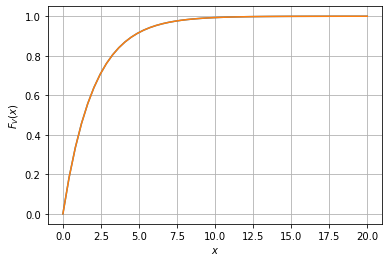
\includegraphics[width=\columnwidth]{./figs/trans/6.1.1.cdf.png}
\caption{CDF of $V$}
\label{fig:probman_trans_cdf_V}
\end{figure}

\begin{figure}[!ht]
\centering
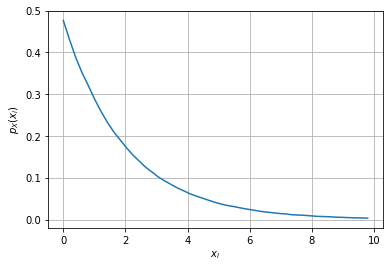
\includegraphics[width=\columnwidth]{./figs/trans/6.1.1.pdf.png}
\caption{PDf of $V$}
\label{fig:probman_trans_PDf_V}
\end{figure}

\item
If
%
\begin{equation}
F_{V}(x) = 
\begin{cases}
1 - e^{-\alpha x} & x \geq 0 \\
0 & x < 0,
\end{cases}
\label{eq:probman_F_V_alpha}
\end{equation}
%
find $\alpha$.
\\
\solution For the value $\alpha=0.5$, the theory matches the simulation.  
The following code generates the CDF of $V$ in Fig. \ref{fig:probman_F_V_alpha} 
Fig. 
\begin{lstlisting}
codes/trans/6.1.2.py
\end{lstlisting}
%
\begin{figure}[!ht]
\centering
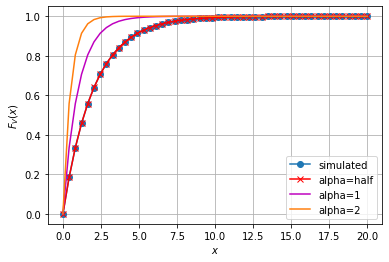
\includegraphics[width=\columnwidth]{./figs/trans/6.1.2.png}
\caption{CDF of $V$}
\label{fig:probman_F_V_alpha}
\end{figure}
%
%
\item
\label{ch3_raleigh_sim}
Plot the CDF and PDf of
%
\begin{equation}
A = \sqrt{V}
\end{equation}
%
\solution The CDF and PDF of A are plotted in Figs. \ref{fig:probman_trans_cdf_A} and \ref{fig:probman_trans_PDf_A}
using the codes below.
\begin{lstlisting}
codes/trans/6.1.3_CDF.py
codes/trans/6.1.3_PDf.py
\end{lstlisting}

\begin{figure}[!ht]
\centering
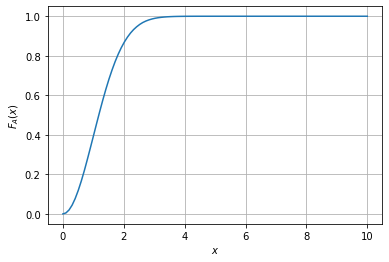
\includegraphics[width=\columnwidth]{./figs/trans/6.1.3.cdf.png}
\caption{CDF of $A$}
\label{fig:probman_trans_cdf_A}
\end{figure}

\begin{figure}[!ht]
\centering
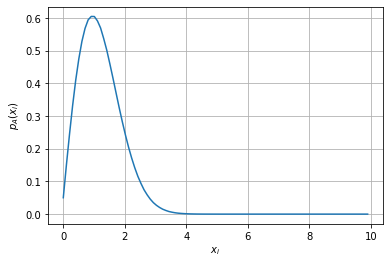
\includegraphics[width=\columnwidth]{./figs/trans/6.1.3.pdf.png}
\caption{PDf of $V$}
\label{fig:probman_trans_PDf_A}
\end{figure}

%
\item
Find an expression for $F_{A}(x)$ using the definition. Plot this expression and compare with the result of problem \ref{ch3_raleigh_sim}. 
\\
\solution 
% Given,
% \begin{align}
% A = \sqrt{V}
% \end{align}

\begin{align} 
F_A(x) &= \pr{A \le x} = \pr{\sqrt{V} \le x}
\\
&= \pr{V \le x^2} = F_V\brak{x^2}
\end{align}
%
From \eqref{eq:probman_F_V_alpha}, 
\begin{align} 
F_V\brak{x^2} = 
\begin{cases}
1 - e^{-\alpha x^2} & x \geq 0 \\
0 & x < 0,
\end{cases}
\end{align}
%
Substituting 

\begin{align}
\alpha = \frac{1}{2}
\end{align}

%
\begin{align} 
F_V\brak{x^2} = 
\begin{cases}
1 - e^{- \frac{x^2}{2}} & x \geq 0 \\
0 & x < 0,
\end{cases}
\end{align}
%
The CDF of A is plotted in Fig. \ref{fig:probman_trans_cdf_A_theory} using the code below.
\begin{lstlisting}
codes/trans/6.1.4.py
\end{lstlisting}
%
\begin{figure}[!ht]
\centering
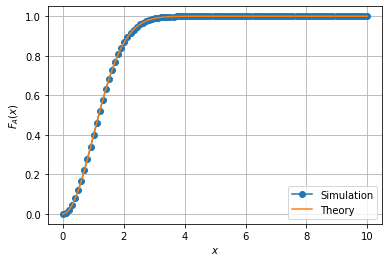
\includegraphics[width=\columnwidth]{./figs/trans/6.1.4.png}
\caption{CDF of $A$}
\label{fig:probman_trans_cdf_A_theory}
\end{figure}
\item
Find an expression for $p_{A}(x)$.
\\
\solution
The PDf is obtained as
\begin{align}
f_V\brak{x^2} &= \frac{d}{dx}F_V\brak{x^2}
\\
&=
\begin{cases}
x e^{- \frac{x^2}{2}} & x \geq 0 \\
0 & x < 0,
\end{cases}
\end{align}
%
The PDf of A is plotted in \ref{fig:probman_trans_pdf_A_theory} using the code below.
\begin{lstlisting}
codes/trans/6.1.5.py
\end{lstlisting}
\begin{figure}[!ht]
\centering
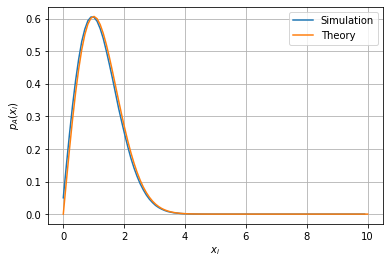
\includegraphics[width=\columnwidth]{./figs/trans/6.1.5.png}
\caption{PDf of $A$}
\label{fig:probman_trans_pdf_A_theory}
\end{figure}
\end{enumerate}

%
\subsection{Using Jacobian}
%
\begin{enumerate}[label=\thesubsection.\arabic*.,ref=\thesubsection.\theenumi]
\numberwithin{equation}{enumi}
\numberwithin{figure}{enumi}

\item
Evaluate the joint PDF of $X_1,X_2$,  given by
%
\begin{equation}
p_{X_1,X_2}(x_1,x_2) = p_{X_1}\brak{x_1}p_{X_2}\brak{x_2}
\end{equation}
%
\solution From \eqref{eq:probman_gauss_pdf}
\begin{align}
p_{X_1}(x_1)&=\frac {1}{\sqrt {2\pi }}e^{-\frac {x_1^2}{2}}
\\
p_{X_2}(x_2)&=\frac {1}{\sqrt {2\pi }}e^{-\frac {x_2^2}{2}}
\\
\implies p_{X_1,X_2}(x_1,x_2) &= \frac {1}{\sqrt {2\pi }}e^{-\frac {x_1^2+x_2^2}{2}}
\label{eq:probman_pdf_x1x2}
\end{align}
 
%
\item
Let 
\begin{align}
 X_1 = \sqrt{V}\cos \theta
\\
 X_2 = \sqrt{V} \sin \theta.
\end{align}
Evaluate the Jacobian 
%
\begin{equation}
J =
\begin{vmatrix}
\frac{\partial x_1}{\partial v} & \frac{\partial x_2}{\partial v} \\
\frac{\partial x_1}{\partial \theta} & \frac{\partial x_2}{\partial \theta} 
\end{vmatrix}
\end{equation}
%
\solution
\begin{align}
J=\begin{vmatrix}
     \frac{1}{2\sqrt{v}}\cos\theta & \frac{1}{2\sqrt{v}}\sin\theta\\
       -v\sin\theta & v\cos\theta
\end{vmatrix}=\frac{1}{2}
\label{eq:probman_jacob_V}
\end{align}
\item
Find
%
\begin{equation}
p_{V,\Theta}\brak{v,\theta} = \abs{J}p_{X_1,X_2}\brak{x_1,x_2}
\end{equation}
%
\solution From \eqref{eq:probman_jacob_V} and \eqref{eq:probman_pdf_x1x2},
\begin{align}
p_{V,\Theta}\brak{v,\theta}=\frac{1}{4\pi}\exp\brak{-\frac{v}{2}}, v \ge 0, 0 < \theta < 2\pi
\label{eq:probman_pdf_V_theta}
\end{align}
%
\item
Find $p_{V}(v)$.
\\
\solution For $v \ge 0$, from \eqref{eq:probman_pdf_V_theta},
\begin{align}
p_{V}(v) &= \int_{0}^{2\pi} \frac{1}{4\pi}\exp\brak{-\frac{v}{2}} d \theta \\
&= \brak{2\pi} \times \frac{1}{4\pi}\exp\brak{-\frac{v}{2}} \\
&= \frac{1}{2}\exp\brak{-\frac{v}{2}}\\
\therefore p_{V}(v) &= 
\begin{cases}
\frac{1}{2}\exp\brak{-\frac{v}{2}} & v\geq 0 \\
0 & v< 0
\end{cases}
\label{eq:probman_pdf_V}
\end{align}
%

\item
Find $p_{\Theta}(\theta)$.  
\\
\solution For $0 \le \theta \le 2\pi$, from \eqref{eq:probman_pdf_V_theta},
\begin{align}
p_{\Theta}(\theta) &= \int_{0}^{\infty} \frac{1}{4\pi}\exp\brak{-\frac{v}{2}} d v \\
&= \frac{1}{2\pi} \left[1 - e^{-\frac{x}{2}} \right]_{0}^{\infty}\\
&= \frac{1}{2\pi}\\
\therefore p_{V}(v) &= 
\begin{cases}
\frac{1}{2\pi} & 0 \leq \theta \leq 2\pi \\
0 & \text{otherwise}
\end{cases}
\end{align}
%
\item
Are $V$ and $\Theta$ independent?
\\
\solution Yes,
\begin{align}
\because p_{V}(v)p_{\Theta}(\theta) &= \frac{1}{2}\exp\brak{-\frac{v}{2}} \times \frac{1}{2\pi}\\
&= \frac{1}{4\pi}\exp\brak{-\frac{v}{2}}\\
&= p_{V,\Theta}\brak{v,\theta}
\end{align}
\item
Find $p_{A}(x)$ using the Jacobian.
\\
\solution 
\begin{align}
p_{A}(x) &= \Pr(A=x) = \Pr(\sqrt{V} = x) \\
&= \Pr(V=x^2) = p_V(x^2)
\end{align}
From \eqref{eq:probman_pdf_V}, as $x^2 \ge 0$,
\begin{align}
p_{V}(x^2) &= \frac{1}{2}\exp\brak{-\frac{x^2}{2}} 
\end{align}
%%
% \item
% Find $p_{V}(v)$.  

% %
% %
% \item
% Find $p_{\Theta}(\theta)$.  

% %
% \item
% Are $Y$ and $\Theta$ independent?

% \item
% Find $p_{A}(x)$ using the Jacobian.

% %%
%\item
%Let $X_1 \sim  \gauss{2}{1}$ and $X_2 \sim  \gauss{3}{1}$. Find $E\sbrak{X_1X_2}$.  Try with different mean and variances. Comment.
%
%

%\section{The Transform Domain}
%\item
%Find the MGF of $X \sim \gauss{\mu}{\sigma^2}$. 
%
%\item
%Find the MGF of $Y$.
%
%%
%\item
%Find the PDF of $Y$ by inverting the MGF.
%
%%
\end{enumerate}

%
\section{Conditional Probability}
\begin{enumerate}[label=\thesection.\arabic*.,ref=\thesection.\theenumi]
\numberwithin{equation}{enumi}
\numberwithin{figure}{enumi}
%%
\item
\label{ch4_sim}
Plot 
\begin{equation}
P_e = \pr{\hat{X} = -1|X=1}
\end{equation}
%
for 
\begin{equation}
Y = AX+N,
\end{equation}
where $A$ is Raleigh with $E\sbrak{A^2} = \gamma, N \sim \gauss{0}{1}, X \in \brak{-1,1}$ for $0 \le \gamma \le 10$ dB.
\\
\solution See Fig. \ref{fig:probman_p_e_gamma}

%
\item
Assuming that $N$ is a constant, find an expression for $P_e$.  Call this $P_e(N)$.
\\
\solution The estimated value $\hat{X}$ is given by
\begin{align}
\hat{X} = 
\begin{cases}
+1 & Y>0\\
-1 & Y<0
\end{cases}
\end{align}
For $X = 1$, 
\begin{align}
Y &= A + N\\
P_e &= \pr{\hat{X} = -1|X=1} \\
&= \pr{Y<0 |X=1}\\
&= \pr{A<-N}\\
&= F_A(-N)\\
&= \int_{-\infty}^{-N} f_A(x)dx
\end{align}
By definition
\begin{align}
f_A(x) = 
\begin{cases}
\frac{x}{\sigma^2}\exp\brak{{-\frac{x^2}{2\sigma^2}}} & x\geq0\\
0 & otherwise
\end{cases}
\end{align}
If $N>0, f_A(x) = 0$. Then,
\begin{align}
 P_e=0  
\end{align}
If $N<0$. Then,
\begin{align}
 P_e(N) &=\int_{-\infty}^{-N} f_A(x)dx\\
 &=\int_{-\infty}^{0} 0dx+\int_{0}^{-N} f_A(x)dx\\
 &=\int_{0}^{-N} \frac{x}{\sigma^2}\exp\brak{{-\frac{x^2}{2\sigma^2}}}dx\\
 &=1-\exp{\brak{-\frac{N^2}{2\sigma^2}}}
\end{align}
Therefore,
\begin{align}\label{pe(N)}
P_e(N) = 
\begin{cases}
1-\exp\brak{{-\frac{N^2}{2\sigma^2}}} & N<0\\
0 & otherwise
\end{cases}
\end{align}
%

%
\item
%
\label{ch4_anal}
For a function $g$,
\begin{equation}
E\sbrak{g(X)} = \int_{-\infty}^{\infty}g(x)p_{X}(x)\, dx
\end{equation}
%
Find $P_e = E\sbrak{P_e(N)}$.
\\
\solution
Since $N \sim \gauss{0}{1}$ ,
\begin{align}
  p_N(x)= \frac{1}{\sqrt{2\pi}}\exp \brak{-\frac{x^2}{2} }\\
\end{align}
And from \eqref{pe(N)} 
\begin{align}
    P_e(x)=
    \begin{cases}
1-\exp\brak{{-\frac{x^2}{2\sigma^2}}} & x<0\\
0 & otherwise
\end{cases}
\end{align}

\begin{align}
 P_e=E\sbrak{P_e(N)} = \int_{-\infty}^{\infty}P_e(x)p_{N}(x)\, dx  
\end{align}
If $x<0, P_e(x)=0$ and using the fact that for an even function
\begin{align}
\int_{-\infty}^{\infty}f(x)=2\int_{-\infty}^{0}f(x)   
\end{align}
we get
\begin{align}
  P_e&= \frac{1}{\sqrt{2\pi}}\int_{-\infty}^{0}\exp \brak{ -\frac{x^2}{2}} \brak{1-\exp \brak{ -\frac{x^2}{2\sigma^2}} } dx\\
&= \frac{1}{2\sqrt{2\pi}} \int_{-\infty}^{\infty} \exp \brak{ -\frac{x^2}{2} }dx \nonumber \\
&- \frac{1}{2\sqrt{2\pi}} \int_{-\infty}^{\infty} \exp \brak{-\frac{(1+ \sigma^2)x^2}{2 \sigma^2}}  dx\\
&= \frac{\sqrt{2\pi} - \sqrt{\frac{\pi(2\sigma^2)}{1+\sigma^2}}}{2\sqrt{2\pi}}\\
&= \frac{1}{2} - \frac{1}{2}\sqrt{\frac{\sigma^2}{1+\sigma^2}}
\end{align}
For a Rayleigh Distribution with scale $= \sigma$,
\begin{align}
E\sbrak{A^2} = 2\sigma^2\\
\gamma = 2\sigma^2\\
\therefore P_e = \frac{1}{2} - \frac{1}{2}\sqrt{\frac{\gamma}{2+\gamma}}
\end{align}
%
%
\item
Plot $P_e$ in problems \ref{ch4_sim} and \ref{ch4_anal} on the same graph w.r.t $\gamma$.  Comment.
\\
\solution $P_e$ is plotted w.r.t $\gamma$ in \ref{fig:probman_p_e_gamma} using the code below.
\begin{lstlisting}
codes/cond/7.4.py
\end{lstlisting}
\begin{figure}[!ht]
\centering
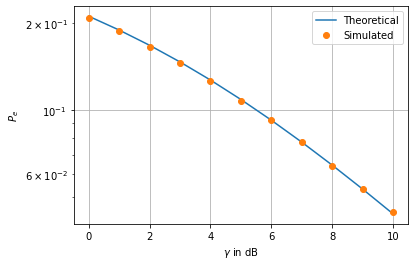
\includegraphics[width=\columnwidth]{figs/cond/7.4.png}
\caption{$P_e$ w.r.t $\gamma$}
\label{fig:probman_p_e_gamma}
\end{figure}
%
\end{enumerate}

%%
\section{Two Dimensions}
\begin{enumerate}[label=\thesection.\arabic*.,ref=\thesection.\theenumi]
\numberwithin{equation}{enumi}
\numberwithin{figure}{enumi}
%%
\item Let 
\begin{equation}
\mbf{y} = A\mbf{x} + \mbf{n},
\end{equation}
where 
\begin{align}
x &\in \brak{\mbf{s}_0,\mbf{s}_1}, 
\mbf{s}_0 = 
\begin{pmatrix}
1 
\\
0
\end{pmatrix},
\mbf{s}_1 = 
\begin{pmatrix}
0 
\\
1
\end{pmatrix}
\\
\mbf{n} &= 
\begin{pmatrix}
n_1
\\
n_2
\end{pmatrix},
n_1,n_2 \sim \gauss{0}{1}.
\end{align}
%
\item
\label{ch5_fsk}
Plot 
%
\begin{equation}
\mbf{y}|\mbf{s}_0 \text{ and } \mbf{y}|\mbf{s}_1
\end{equation}
%
on the same graph using a scatter plot.
%
\solution The following python code plots the scatter plot when $\mbf{x} = \mbf{s}_0$ and $\mbf{x} = \mbf{s}_1$ in Fig. \ref{fig:scatter_plt_y}
\begin{lstlisting}
codes/twoD/scatter_plot.py
\end{lstlisting}
\begin{figure}
\centering
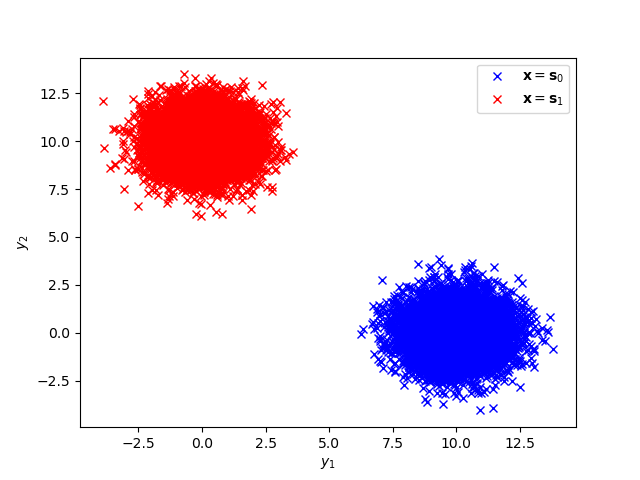
\includegraphics[width=\columnwidth]{./figs/twoD/scatter_plot.png}
\caption{Scatter plot of $\mbf{y} = \begin{pmatrix} y_1 \\ y_2 \end{pmatrix}$ for $A = 10$}
\label{fig:scatter_plt_y}
\end{figure}
%
%
\item
For the above problem, find a decision rule for detecting the symbols $\mbf{s}_0 $ and $\mbf{s}_1$.
\\
\solution The multivariate Gaussian distribution is defined as
%
\begin{multline}
\label{eq:multivariate}
p_{\mathbf{x}}(x_1,\dots,x_k)
\\
=\frac{1}{\sqrt{\brak{2\pi}^k\abs{\mbf{\Sigma}}}}\exp\cbrak{-\frac{1}{2}\brak{\mathbf{x}-\mbf{\mu}}^T\mbf{\Sigma}^{-1}\brak{\mathbf{x}-\mbf{\mu}}}
\end{multline}
%
where $\mbf{\mu}$ is the mean vector, $\mbf{\Sigma} = E\sbrak{\brak{\mathbf{x}-\mbf{\mu}}\brak{\mathbf{x}-\mbf{\mu}}^T}$ is the covariance matrix and $\abs{\mbf{\Sigma}}$ is the determinant of $\mbf{\Sigma}$.
For a bivariate gaussian distribution,
{\small
\begin{multline}
\label{eq:bivariate}
p(x,y)= \frac{1}{2\pi \sigma_x\sigma_y\sqrt{1-\rho^2}}\exp\lsbrak{-\frac{1}{2\brak{1-\rho^2}}}
\\
\times \rsbrak{\cbrak{\frac{\brak{x-\mu_x}^2}{\sigma_x^2}+\frac{\brak{y-\mu_y}^2}{\sigma_y^2}-\frac{2\rho\brak{x-\mu_x}\brak{y-\mu_y}}{\sigma_x\sigma_y}}}
\end{multline}
}
%
where
%
\begin{align}
%\mbf{\mu}=
&\mbf{\mu}=
\begin{pmatrix*}
\mu_x \\
\mu_y
\end{pmatrix*},
\mbf{\Sigma} = 
\begin{pmatrix*}%[r]
\sigma_x^2 & \rho\sigma_x\sigma_y \\
\rho\sigma_x\sigma_y & \sigma_y^2
\end{pmatrix*},\\
&\rho = \frac{E\sbrak{\brak{x - \mu_x}\brak{y-\mu_y}}}{\sigma_x\sigma_y}.
\end{align}
%
\begin{align}
    \mbf{y}|s_0 &= 
    \begin{pmatrix}
    A+n_1 \\
    n_2
    \end{pmatrix}\\
    \mbf{y}|s_1 &=  
    \begin{pmatrix}
    n_1 \\
    A+n_2
    \end{pmatrix}
    \end{align}
    Substituting these values in (\ref{eq:bivariate}),
    \begin{multline}
    \label{gauss_mutl_var1}
    p\brak{\mbf{y}|s_0} = \frac{1}{2\pi\sigma_{y_1}\sigma_{y_2}\sqrt{1-\rho_1^2}}\exp\lsbrak{-\frac{1}{2\brak{1-\rho_1^2}}}
    \\
    \times \rsbrak{\cbrak{\frac{\brak{y_1-A}^2}{\sigma_{y_1}^2}+\frac{\brak{y_2}^2}{\sigma_{y_2}^2}-\frac{2\rho_1\brak{y_1-A}\brak{y_2}}{\sigma_{y_1}\sigma_{y_2}}}}
    \end{multline}
    \begin{multline}
    \label{gauss_mutl_var2}
    p\brak{\mbf{y}|s_1} = \frac{1}{2\pi\sigma_{y_1}\sigma_{y_2}\sqrt{1-\rho_2^2}}\exp\lsbrak{-\frac{1}{2\brak{1-\rho_2^2}}}
    \\
    \times \rsbrak{\cbrak{\frac{\brak{y_1}^2}{\sigma_{y_1}^2}+\frac{\brak{y_2-A}^2}{\sigma_{y_2}^2}-\frac{2\rho_2\brak{y_1}\brak{y_2-A}}{\sigma_{y_1}\sigma_{y_2}}}}
    \end{multline}
    where,
    \begin{align}
    \label{rho_sig_val}
    \rho_1 = E[(y_1-A)(y_2)] &= E[n_1 n_2] = 0, \nonumber \\
    \rho_2 = E[(y_1)(y_2-A)] &= E[n_1 n_2] = 0, \nonumber \\
    \sigma_{y_1} = \sigma_{y_2} &= 1
    \end{align}
    For equiprobably symbols, the MAP criterion is defined as
    %
    \begin{align}
    \label{eq:map_bfsk_dec}
    p\brak{\vec{y}|s_0} &\dec{s_0}{s_1} p\brak{\vec{y}|s_1}
    \end{align}
    Using (\ref{gauss_mutl_var1}) and (\ref{gauss_mutl_var2}) and substituting the values from (\ref{rho_sig_val}),  we get
    \begin{align}
    (y_1 -A)^2 + y_2^2 \dec{s_1}{s_0} y_1^2 + (y_2 - A)^2
    \end{align}
    On simplifying, we get the decision rule is
    \begin{align}
    \label{eq:decision_rule}
    y_1 \dec{s_0}{s_1} y_2
    \end{align}
%    
\item
Plot 
\begin{equation} 
P_e = \pr{\hat{\mbf{x}} = \mbf{s}_1|\mbf{x} = \mbf{s}_0}
\end{equation}
with respect to the SNR from 0 to 10 dB.
\\
\solution
\begin{figure}
    \centering
    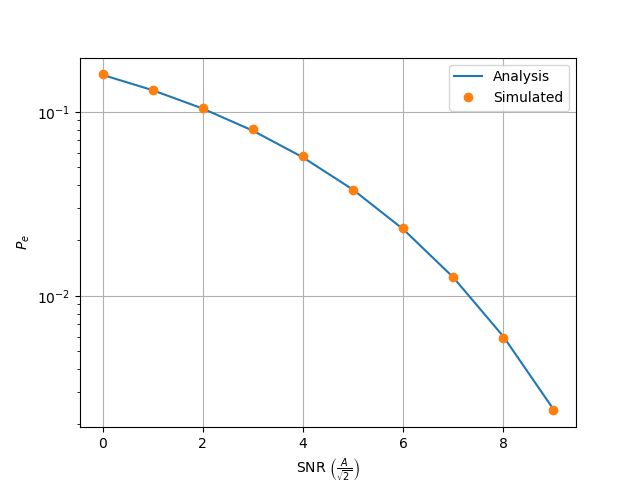
\includegraphics[width=\columnwidth]{./figs/twoD/ber_snr_plot.png}
    \caption{$P_e$ with respect to SNR from 0 to 10 dB}
    \label{fig:ber_snr_plot}
    \end{figure}
%
\item
Obtain an expression for $P_e$. Verify this by comparing the theory and simulation plots on the same graph.
\\
\solution 
\begin{align}
P_e = \pr{\hat{\mbf{x}} = \mbf{s}_1|\mbf{x} = \mbf{s}_0}
\end{align}
Given that $\mbf{s}_0$ was transmitted, the received signal is
\begin{align}
\mbf{y}|\mbf{s}_0 = \begin{pmatrix} A \\ 0 \end{pmatrix} + \begin{pmatrix} n_1 \\ n_2 \end{pmatrix}
\end{align}
From (\ref{eq:decision_rule}), the probability of error is given by 
\begin{align}
P_e &= \pr{y_1 < y_2 |\mbf{s}_0} = \pr{A+n_1 < n_2}\\
&= \pr{n_2 - n_1 > A}
\end{align}
Note that $n_2 - n_1 \sim \gauss{0}{2}$. Thus,
\begin{align}
P_e &= \pr{\sqrt{2}w > A}\\
\pr{w > \dfrac{A}{\sqrt{2}}}\\
\Rightarrow P_e &= \qfunc{\frac{A}{\sqrt{2}}}
\end{align}
where $w \sim \gauss{0}{1}$. The following code plots the $P_e$ curve in Fig. (\ref{fig:ber_snr_plot}).
\begin{lstlisting}
codes/twoD/ber_snr_plot.py
\end{lstlisting}
%
\end{enumerate}

%%
\section{Transform Domain: Moment Generating Function}
Let $X \sim \gauss{\mu}{\sigma^2}$.

\begin{enumerate}[label=\thesection.\arabic*.,ref=\thesection.\theenumi]
\numberwithin{equation}{enumi}
\numberwithin{figure}{enumi}
%%
\item
Find $M_{X}\brak{s} = E\sbrak{e^{-sX}}$.
\\
\solution The MGF of $X$ is
%
\begin{align}
M_{X}(s) &=\int_{-\infty}^{\infty}e^{-s X}p_{X}(x) dx 
\\
&=e^{-s\mu}e^{-\frac{s^2\sigma^2}{2}}
\label{eq:probman_mgf_X}
\end{align}
%
\item
Let 
%
\begin{equation}
N = n_1 - n_2, \quad   n_1,n_2 \sim \gauss{0}{1}.
\end{equation}
%
Find $M_{N}(s)$, assuming that $n_1$ and $n_2$ are independent.
\\
\solution Substituting from \eqref{eq:probman_mgf_X} and using independence,
\begin{align}
M_N(s)&=E[e^{-(n_1-n_2)s}]=M_{n_1}(s) M_{n_2}(-s)
\\
&= e^{-s^2\sigma^2} = e^{-s^2} \quad \brak{\because \sigma = 1}
\label{eq:probman_mgf_N}
\end{align}
%
\item
Show that $N$ is Gaussian. Find its mean and variance.  Comment.
\\
\solution From \eqref{eq:probman_mgf_N} and \eqref{eq:probman_mgf_X}, it is obvious that $X \sim \gauss{0}{2}$.  Thus,
%
the difference of two Gaussian random variables is also a Gaussian random variable.

\end{enumerate}

%%
\section{Uniform to Other: Quantile function}
\begin{enumerate}[label=\thesection.\arabic*.,ref=\thesection.\theenumi]
\numberwithin{equation}{enumi}
\numberwithin{figure}{enumi}
%%
%
%
\item
Generate samples of 
%
\begin{equation}
V = -2\ln\brak{1-U}
\label{eq:probman_V_cdf_sim}
\end{equation}
%
and plot its CDF.  Comment.
\\
\solution
%
\begin{align}
    E(X) &= \frac{1}{\sqrt{2\pi}} \int_{-\infty}^{\infty} x e^{-\frac{x^2}{2}}dx\\
    &=0 \quad \brak{ \text{ odd function}}
\end{align}
\begin{align}
    E\brak{X^2}&= \frac{1}{\sqrt{2\pi}}\int_{-\infty}^{\infty} x^2
e^ {-\frac{x^2}{2}} dx \quad \brak{even function}\\
    &= \frac{2}{\sqrt{2\pi}} \int_{0}^{\infty} x^2 e^{-\frac{x^2}{2}} dx\\
    &= \frac{2}{\sqrt{2\pi}}\int_{0}^{\infty}\sqrt{2u}e^{-u} du \quad\brak{Let \frac{x^2}{2}= u}\\
    &= \frac{2}{\sqrt{\pi}} \int_{0}^{\infty} e^{-u} u^{\frac{3}{2}-1} du\\
    &= \frac{2}{\sqrt{\pi}} \Gamma\brak{{\frac{3}{2}}}\\
    &= \frac{1}{\sqrt{\pi}}\Gamma\brak{\frac{1}{2}} \\
    &= 1
\end{align}
where we have used the fact that
\begin{align}
\quad\because \Gamma(n)= (n-1)\Gamma(n-1); \Gamma\brak{\frac{1}{2}}=\sqrt{\pi}
\end{align}
%
Thus, the  variance is
\begin{align}
    \sigma^2 =  E\brak X^2 - E^2\brak X = 1
\end{align}


%
\item
Generate the Rayleigh distribution from Uniform. Verify your result through graphical plots.

\end{enumerate}

\section{Miscellaneous Distributions}
\begin{enumerate}[label=\thesection.\arabic*.,ref=\thesection.\theenumi]
\numberwithin{equation}{enumi}
\numberwithin{figure}{enumi}

\item A carton consists of 100 shirts of which 88 are good, 8 have minor defects and 4 have major defects.Jimmy, a trader, will only accept the shirts which are good, but Sujatha, another trader, will only reject the shirts which have major defects.One shirt is drawn at random from the carton. What is the probability that\\
(i) it is acceptable to Jimmy?\\
(ii) it is acceptable to Sujatha?
\\
\solution
From the given information, Table \ref{table:5.19} can be generated.
\begin{table}[!ht]
\centering
\resizebox{\columnwidth}{!}{
\begin{tabular}{|p{4cm}|p{4cm}|}
\hline
\multicolumn{2}{|c|}{\textbf{A Random variable which has 3 possible values}}\\ \hline
\multirow{2}{*}{$\pr{X=0}=\frac{4}{100}=0.04$} & out of 100, 4 have major defects shirts
\\
\hline
\multirow{2}{*}{$\pr{X=1}=\frac{8}{100}=0.08$} & out of 100,8 are accepted minor defected shirts\\ \hline
\multirow{2}{*}{$\pr{X=2}=\frac{88}{100}=0.88$} & out of 100,88 are accepted good shirts\\ \hline
\end{tabular}
}
\caption{Random variables}
\label{table:5.19}
\end{table}
Then
\begin{enumerate}
\item The probability that the shirt is acceptable to Jimmy is
\begin{align}
\pr{X=2}=\frac{88}{100}
\end{align}
%
\item The probability that the shirt is acceptable to Sujatha is
\begin{align}
1-\pr{X=0}=1-\frac{4}{100} = \frac{96}{100}
\end{align}

\end{enumerate}
%
The following code simulates the probability
\begin{lstlisting}
codes/misc/discrete.ipynb
\end{lstlisting}
\end{enumerate} 

%\section{Sum of i.i.d random variables}
%\input{./chapters/conv.tex}


\end{document}


